% =============================================================================
% COMP9444 Group Project 047 -- Breast Cancer Classification and Segmentation
% Detailed report: Introduction, Literature Review, Dataset & EDA, Models & Methods,
% Experimental Setup, Results, Discussion, Conclusion.
%
% Sources of truth: COMP9444_EDA.ipynb and Models/results/*.json.
% Every numerical value below is traceable to those files.
%
% Figures: this file expects the PNGs in ./figures/ (already populated). The
% \graphicspath below also searches Models/results/figures/ and EDA/figures/.
% Compiles on Overleaf and with local pdflatex/MiKTeX as-is.
% =============================================================================
\documentclass[11pt]{article}

\usepackage[utf8]{inputenc}
\usepackage[T1]{fontenc}
\usepackage[margin=1in]{geometry}
\usepackage{amsmath,amssymb}
\usepackage{graphicx}
\usepackage{booktabs}
\usepackage{tabularx}
\usepackage{array}
\usepackage{multirow}
\usepackage{subcaption}
\usepackage{xcolor}
\usepackage{float}
\usepackage{cite}
\usepackage{hyperref}
\hypersetup{colorlinks=true, linkcolor=black, citecolor=blue, urlcolor=blue}
\graphicspath{{figures/}{Models/results/figures/}{EDA/figures/}}

% Long \texttt{} paths/package names cannot hyphenate and would otherwise stick
% out into the margin; give TeX some slack rather than breaking them by hand.
\emergencystretch=3em

% convenience column types for tabularx
\newcolumntype{L}[1]{>{\raggedright\arraybackslash}p{#1}}
\newcolumntype{Y}{>{\raggedright\arraybackslash}X}
\newcommand{\best}[1]{\textbf{#1}}

\title{Breast Cancer Classification and Segmentation\\
Using Deep Learning on Ultrasound Images:\\
A Leakage-Free Benchmark, an Improved Segmenter, and a Rigorously\\
Evaluated Segmentation-Guided Classifier}
\author{COMP9444 Group AreuOk? Project 047}
\date{}

\begin{document}
\maketitle

\begin{abstract}
\noindent
Breast ultrasound (BUS) is a safe, low-cost imaging modality for breast-cancer
screening, but it is difficult to interpret and its main public benchmark,
BUSI, is small, imbalanced and contains many near-duplicate images. We study
lesion \emph{segmentation} and image \emph{classification} on BUSI under a
single, carefully cleaned, \emph{leakage-free} evaluation protocol. Using
perceptual hashing we find that roughly one third of BUSI images belong to
near-duplicate clusters and that an exact cross-class duplicate exists; we
therefore split the data at the cluster level. Under this protocol we reproduce
thirteen published models and add two of our own: an improved pretrained-encoder
U-Net and an improved segmentation-guided (dual-stage) classifier. A controlled
ablation shows that an ImageNet-pretrained encoder alone raises segmentation Dice
from $0.648$ to $0.765$ and is responsible for essentially all of our
segmenter's gain, whereas a Focal-Tversky loss, test-time augmentation and
attention gates do not reliably improve overlap. A controlled Stage-1
substitution shows the dual-stage pipeline is limited by its \emph{classifier},
not its segmenter. When candidate classifier improvements are evaluated
rigorously (out-of-fold training masks, five-seed ensembling and bootstrap
$95\%$ confidence intervals), hand-crafted shape/radiomics features give no
reliable gain and only ensembling survives, reaching macro-F1 $0.875$
($95\%$ CI $[0.80,0.94]$). Our reproductions of published BUSI models score
below their reported numbers, which we attribute to removing near-duplicate
leakage. This is an experimental decision-support study, not a system for
autonomous clinical diagnosis.
\end{abstract}

% =============================================================================
\section{Introduction}
\label{sec:intro}
% =============================================================================
Breast cancer is one of the leading causes of cancer-related death among women
worldwide, and early detection remains the single most effective way to reduce
mortality and improve outcomes~\cite{cheng2010survey,xian2018survey}. Among the
common imaging modalities, breast ultrasound (BUS) is safe, inexpensive and
radiation-free, and is particularly valuable for younger patients and for dense
breast tissue, where the sensitivity of mammography is reduced.

Despite these advantages, BUS images are hard to read. They suffer from
\emph{speckle noise}, \emph{low contrast}, \emph{acoustic shadowing} and
\emph{blurred lesion boundaries}, and the appearance of a lesion (its shape,
echogenicity and texture) varies greatly between and within the benign and
malignant categories~\cite{xian2018survey,aldhabyani2020busi}. As a result,
manual assessment is slow and operator-dependent, with appreciable
inter-observer variability. Several BUSI images additionally contain
\emph{burned-in annotations}, calipers and text (for example ``RT LOQ'' or
``RIGHT BREAST''), which a model could exploit as a spurious shortcut. These
difficulties motivate computer-aided diagnosis (CAD) systems that can support,
rather than replace, the radiologist.

Classification and segmentation are complementary views of the same clinical
problem. \emph{Classification} answers \emph{what} a scan shows -- normal tissue,
a benign mass, or a malignant mass -- while \emph{segmentation} answers
\emph{where} the lesion is, delineating its boundary at the pixel level. A
lesion mask supports interpretability and downstream measurement, and it can be
used to focus a classifier on the lesion rather than on surrounding clutter,
which links the two tasks in a single pipeline.

\paragraph{Problem statement.}
Following the Project~047 brief, we build and evaluate a deep-learning system on
the Breast Ultrasound Images (BUSI) dataset~\cite{aldhabyani2020busi} that
addresses both tasks: three-class classification
(\texttt{normal}/\texttt{benign}/\texttt{malignant}) and binary lesion
segmentation. Our central concern is \emph{trustworthy comparison}: BUSI is
small, imbalanced and, as we show, riddled with near-duplicate images, so a
careless evaluation can substantially inflate reported scores. We therefore
build a single cleaned, leakage-free evaluation protocol and compare every model
under it.

\paragraph{Research questions.}
The study is organised around four questions.
\begin{itemize}
  \item \textbf{RQ1.} How do established segmentation and classification
  architectures perform under a common, leakage-free BUSI evaluation protocol,
  and how do those numbers compare with the values reported in the original
  papers?
  \item \textbf{RQ2.} Which design decisions most strongly affect segmentation
  performance on the small BUSI dataset (transfer learning, loss function,
  attention, inference-time processing)?
  \item \textbf{RQ3.} Does improving lesion segmentation reliably improve
  downstream segmentation-guided classification?
  \item \textbf{RQ4.} Are apparent improvements stable across random seeds and
  statistical resampling, or are they artefacts of a single training run on a
  small test set?
\end{itemize}

\paragraph{Contributions.}
Grounded in the actual work, our contributions are:
(i)~a near-duplicate analysis of BUSI (perceptual hashing and cluster detection)
and a \emph{cluster-grouped, class-stratified} leakage-free split;
(ii)~a unified reproduction of thirteen published models -- eight segmentation
architectures, three classification backbones, one dual-stage pipeline and one
multi-task network -- all trained and evaluated under this one protocol;
(iii)~an improved pretrained-encoder segmenter with a \emph{controlled ablation}
that isolates the contribution of each ingredient;
(iv)~an improved dual-stage (segmentation-guided) classifier, including a
controlled Stage-1 substitution and a ground-truth-ROI upper-bound diagnostic;
and
(v)~a \emph{rigorous evaluation protocol} for the dual-stage system that uses
out-of-fold training-mask generation, multi-seed ensembling and bootstrap
$95\%$ confidence intervals, which we use to separate real improvements from
noise.

\paragraph{Report organisation.}
Section~\ref{sec:litreview} reviews related work and identifies the gaps this
project targets. Section~\ref{sec:eda} describes the dataset and our exploratory
data analysis (EDA), and maps each observation to a modelling decision.
Section~\ref{sec:models} details the models, our own components and the loss
functions. Section~\ref{sec:setup} specifies the experimental setup: splits,
hyper-parameters, metrics and the statistical protocol. Section~\ref{sec:results}
reports results and error analysis, Section~\ref{sec:discussion} discusses their
implications and limitations, and Section~\ref{sec:conclusion} concludes.

% =============================================================================
\section{Literature Review}
\label{sec:litreview}
% =============================================================================
We organise the literature thematically and then synthesise the gaps that
motivate our methodology.

\subsection{Breast-ultrasound CAD and the BUSI dataset}
Classical CAD for breast ultrasound followed a pipeline of pre-processing,
segmentation, feature extraction and classification; the surveys of Cheng et
al.~\cite{cheng2010survey} and Xian et al.~\cite{xian2018survey} review two
decades of such methods and recur to the same difficulties -- speckle noise, low
signal-to-noise ratio, low contrast and fuzzy boundaries -- that still dominate
today. The public BUSI dataset of Al-Dhabyani et
al.~\cite{aldhabyani2020busi} has become the de-facto benchmark, providing
\texttt{normal}/\texttt{benign}/\texttt{malignant} images with pixel-level masks
and thus supporting both tasks. Because BUSI is small, augmentation matters: the
same authors showed that traditional and GAN-based augmentation improve
classification on breast ultrasound~\cite{aldhabyani2019augmentation}. Crucially,
a documented data-quality issue -- repeated and near-duplicate frames, some with
conflicting labels -- has been raised for BUSI~\cite{pawlowska2023}; we quantify
this directly in Section~\ref{sec:eda-dup} and design our evaluation around it.

\subsection{CNN-based classification}
Modern image classification is dominated by deep convolutional backbones.
ResNet~\cite{he2016resnet} introduced residual (identity-shortcut) connections
that make very deep networks trainable; DenseNet~\cite{huang2017densenet}
connects each layer to all subsequent layers, promoting feature reuse and
parameter efficiency, which is attractive for small datasets; and
EfficientNet~\cite{tan2019efficientnet} uses compound scaling of depth, width
and resolution to reach high accuracy at low cost, with its smaller variants
(B0/B1) transferring well to medical data. These backbones have been applied
directly to BUSI: Latha et al.~\cite{latha2024effnetb7} fine-tuned
EfficientNet-B7 with heavy pre-processing and Grad-CAM~\cite{selvaraju2017gradcam}
explainability and reported very high accuracy (around $99\%$); such near-perfect
numbers on so small a dataset must be treated cautiously because of possible data
leakage, an observation that directly motivates our protocol.

\subsection{U-Net-based segmentation}
The U-Net~\cite{ronneberger2015unet} encoder--decoder with skip connections is
the foundational biomedical-segmentation architecture and trains well from few
annotated images. Refinements include UNet++~\cite{zhou2018unetpp}, which adds
nested dense skip pathways with deep supervision to bridge the encoder--decoder
semantic gap, and UNet~3+~\cite{huang2020unet3plus}, which fuses features at full
scale. Yap et al.~\cite{yap2018cnn} were among the first to apply deep learning
to BUS lesion detection, comparing a patch-based LeNet, a U-Net, and a
transfer-learned fully convolutional AlexNet (FCN-AlexNet), with the FCN
performing best.

\subsection{Attention and multi-scale segmentation}
Attention U-Net~\cite{oktay2018attentionunet} inserts additive attention gates on
the skip connections so the network learns \emph{where to look}, suppressing
irrelevant background. From semantic segmentation, DeepLabV3+~\cite{chen2018deeplabv3plus}
combines atrous (dilated) separable convolutions and Atrous Spatial Pyramid
Pooling (ASPP) for multi-scale context with a light decoder. TransUNet~\cite{chen2021transunet}
couples a Transformer encoder with a U-Net decoder to model long-range
dependencies, but Transformers are typically data-hungry and require large-scale
pre-training. Two architectures are tailored to BUS: AAU-Net~\cite{chen2023aaunet}
replaces standard convolutions with a hybrid adaptive attention module for
blurred boundaries and irregular malignant shapes, and CResU-Net~\cite{derakhshandeh2024cresunet}
schedules specialised residual/dense encoder blocks and reports the strongest
BUSI Dice in this literature.

\subsection{Transfer learning and self-configuring pipelines}
Transfer learning from ImageNet is a standard remedy for small medical datasets,
reusing general low-level features and stabilising optimisation. nnU-Net~\cite{isensee2021nnunet}
is a self-configuring U-Net pipeline that automatically selects pre-processing,
architecture and training and remains a strong medical-segmentation baseline. The
Segment Anything Model (SAM)~\cite{kirillov2023sam} and its medical adaptation
MedSAM~\cite{ma2024medsam} are promptable foundation segmenters with strong
zero-shot transfer; they are trained mostly on natural or general medical images
and typically require prompts or adaptation, so we treat them as context rather
than as baselines.

\subsection{Joint and dual-stage segmentation--classification}
Most relevant to our combined system are methods that address both tasks. Bruno
et al.~\cite{bruno2025dualstage} propose a \emph{sequential} dual-stage
framework: a segmentation network localises the lesion, a region of interest
(ROI) is cropped from the predicted mask, and a compact CNN then classifies the
ROI as benign or malignant. Lu et al.~\cite{lu2025multitask} instead use
\emph{joint} multi-task learning with a shared encoder and separate segmentation
(object-contextual-attention) and classification heads. These two lines --
sequential and joint -- frame the design space we explore.

\subsection{Evaluation weaknesses in small medical-imaging datasets}
A recurring methodological weakness underlies much of this literature. Reported
BUSI scores are often obtained with different splits and pre-processing,
preventing fair comparison; many studies report a \emph{single} training run
without seeds or confidence intervals; and near-duplicate images can leak between
train and test under a naive split, inflating scores. On a test set as small as
BUSI's, single-run differences of a few points may not be statistically
resolved. These weaknesses are precisely what our protocol addresses.

\begin{table}[t]
\centering
\caption{Comparative summary of the most relevant prior work. ``Reported result''
lists a paper-stated BUSI number where available to us; ``n/r'' = not reported
(to us). Values are as stated by the cited works, not re-measured here.}
\label{tab:litcompare}
\footnotesize
\begin{tabularx}{\linewidth}{@{}l l l Y c Y@{}}
\toprule
Ref & Yr & Task & Key architecture / idea & Reported (BUSI) & Limitation for this project \\
\midrule
BUSI~\cite{aldhabyani2020busi}        & 2020 & Both & Dataset + masks (n/a)                     & n/a    & Small; near-duplicates; imbalance \\
Yap~\cite{yap2018cnn}                 & 2018 & Seg/Det & Patch-LeNet, U-Net, FCN-AlexNet        & n/r    & Detection focus; not BUSI; older nets \\
U-Net~\cite{ronneberger2015unet}      & 2015 & Seg  & Encoder--decoder + skip connections      & n/r    & Not BUS-specific; no speckle handling \\
DeepLabV3+~\cite{chen2018deeplabv3plus}& 2018 & Seg  & ASPP + atrous separable conv             & n/r    & Natural-image net; tuning for BUS \\
Attn.\ U-Net~\cite{oktay2018attentionunet}& 2018 & Seg & Additive attention gates on skips        & n/r    & Designed for CT; adds complexity \\
AAU-Net~\cite{chen2023aaunet}         & 2023 & Seg  & Hybrid adaptive attention (BUS)          & Dice $0.775$ & Complex; costly to reproduce faithfully \\
CResU-Net~\cite{derakhshandeh2024cresunet}& 2024 & Seg & Co-Block / residual block schedule (BUS) & Dice $0.829$ & Reported CV without de-duplication \\
nnU-Net~\cite{isensee2021nnunet}      & 2021 & Seg  & Self-configuring U-Net pipeline          & n/r    & Compute-heavy; general (not BUS) \\
ResNet~\cite{he2016resnet}            & 2016 & Cls  & Residual shortcuts                       & n/r    & Natural-image backbone; overfits small data \\
DenseNet~\cite{huang2017densenet}     & 2017 & Cls  & Dense connectivity / feature reuse       & n/r    & As above; needs regularisation \\
EfficientNet~\cite{tan2019efficientnet}& 2019 & Cls  & Compound scaling (MBConv)                & n/r    & High-capacity variants overfit BUSI \\
Bruno~\cite{bruno2025dualstage}       & 2025 & Both & Dual-stage seg $\rightarrow$ ROI $\rightarrow$ cls & Dice $0.769$; F1 $0.944$ & 2-class; pipeline more complex \\
MTL-OCA~\cite{lu2025multitask}        & 2025 & Both & Shared encoder + OCA + cls head          & n/r    & Details/numbers to confirm; shares capacity \\
\bottomrule
\end{tabularx}
\end{table}

\subsection{Research gaps and project motivation}
\label{sec:gaps}
Synthesising the above, six gaps motivate this project and connect directly to
our methodology. First, \textbf{BUSI is small and imbalanced}, so results are
sensitive to overfitting and to the choice of metric; we therefore use transfer
learning, class-weighted losses and macro-averaged metrics. Second,
\textbf{near-duplicate images cause train/test leakage}; we detect duplicates and
split at the cluster level (Section~\ref{sec:eda-dup}). Third, \textbf{published
models use different splits and pre-processing}, preventing fair comparison; we
put every model through one shared pipeline. Fourth, \textbf{many studies report
a single run}; we report multi-seed statistics for our final pipeline. Fifth,
\textbf{confidence intervals are usually absent}; we add bootstrap $95\%$ CIs.
Sixth, \textbf{it is unclear whether better segmentation implies better
downstream classification}; we test this directly with a controlled Stage-1
substitution and a ground-truth-ROI upper bound. Finally, because high published
BUSI scores may not survive a leakage-free split, we expect -- and report -- our
reproductions to be lower but more trustworthy.

% =============================================================================
\section{Dataset and Exploratory Data Analysis}
\label{sec:eda}
% =============================================================================
All EDA numbers in this section are computed in \texttt{COMP9444\_EDA.ipynb}
(Sections~2--3) from a cached per-image metadata table; we quote them here and
connect each observation to a modelling decision.

\subsection{Dataset composition}
\label{sec:eda-comp}
BUSI~\cite{aldhabyani2020busi} was collected in 2018 at Baheya Hospital, Cairo,
from $600$ female patients aged $25$--$75$. It contains $780$ grayscale
ultrasound scans stored as PNG (average size $\approx 500\times500$\,px), each
with an image-level label in \{\texttt{normal}, \texttt{benign},
\texttt{malignant}\} and one or more pixel-level ground-truth lesion masks;
\texttt{normal} scans carry an all-black mask. Table~\ref{tab:overview}
summarises the dataset. Every image has at least one mask (no orphan files), and
$647$ images contain a real (non-empty) lesion.

A small number of images ship with \emph{multiple} mask files (17 images, up to
three masks each, mostly benign). For binary segmentation we merge these into a
single target by pixel-wise \emph{union} (\texttt{eda\_utils.load\_union\_mask}).
We use the data in three ways: \textbf{three-class classification} uses all
classes; \textbf{lesion segmentation} uses only the benign+malignant images that
contain a lesion; and the \textbf{two-class dual-stage} classifier operates on the
benign/malignant lesion images. The exact split counts are given in
Section~\ref{sec:setup}.

\begin{table}[t]
\centering
\caption{BUSI overview (computed in the notebook). ``Images with a real lesion''
excludes \texttt{normal} scans, whose masks are empty.}
\label{tab:overview}
\small
\begin{tabular}{@{}lc@{\hspace{2em}}lc@{}}
\toprule
Property & Value & Property & Value \\
\midrule
\# images            & $780$          & Images with $\geq 1$ mask   & $780$ \\
\# classes           & $3$            & Images with a real lesion   & $647$ \\
Class names          & n/b/m          & Images with multiple masks  & $17$ (max $3$) \\
Unique image sizes   & $639$          & Width range (px)            & $190$--$1048$ \\
Channels (stored)    & RGB ($780$)    & Height range (px)           & $310$--$719$ \\
\bottomrule
\end{tabular}
\end{table}

\subsection{Class imbalance}
\label{sec:eda-imb}
The classes are imbalanced (Fig.~\ref{fig:classdist}): \texttt{benign} $437$
($56.0\%$), \texttt{malignant} $210$ ($26.9\%$) and \texttt{normal} $133$
($17.1\%$); benign is roughly three times the size of normal. Under such
imbalance, plain accuracy is misleading -- a classifier can score highly by
favouring the majority class -- so we report \emph{macro-averaged} F1 and
one-vs-rest ROC-AUC as primary metrics, together with per-class
precision/recall/F1 and the confusion matrix. Because missing a malignant case is
the costliest error, we pay particular attention to \emph{malignant recall}. The
imbalance also motivates a \emph{stratified} split and an \emph{inverse-frequency
class-weighted} loss (Section~\ref{sec:losses}). We expect the malignant and
normal classes to be harder: malignant is a minority and visually variable, and
normal (no lesion) can be confused with subtle benign findings.

\begin{figure}[t]
\centering
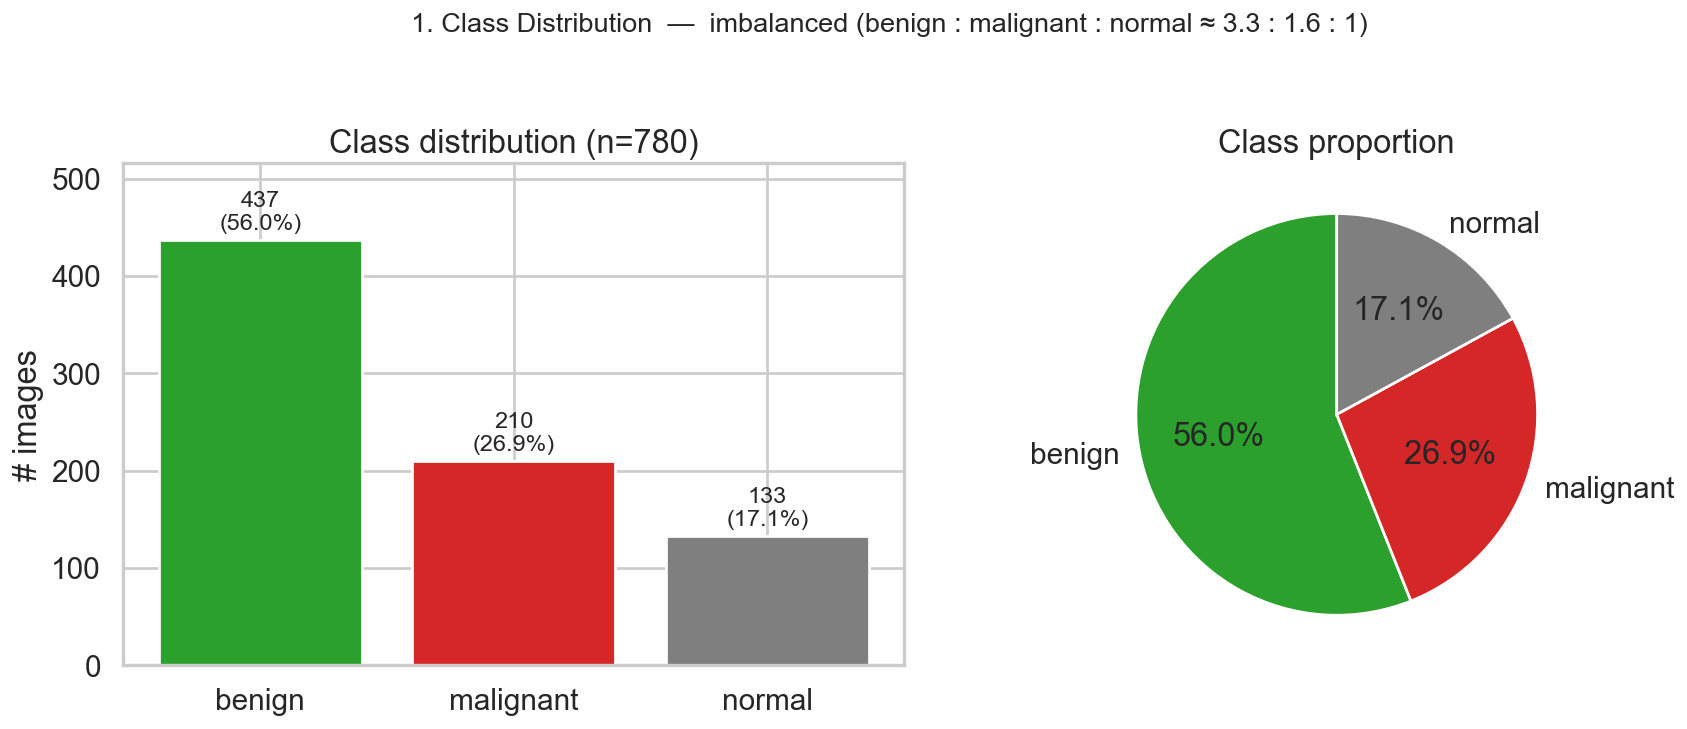
\includegraphics[width=0.86\linewidth]{fig01_class_distribution}
\caption{Class distribution of BUSI ($n=780$). The dataset is imbalanced
(benign:malignant:normal $\approx 3.3:1.6:1$), which drives our use of class
weighting and macro-averaged metrics rather than raw accuracy.}
\label{fig:classdist}
\end{figure}

\subsection{Image dimensions, channels and intensity}
\label{sec:eda-img}
Image sizes vary widely -- $639$ distinct resolutions, width $190$--$1048$\,px and
height $310$--$719$\,px -- and most images are landscape ($W/H>1$)
(Fig.~\ref{fig:imgsize}). Although ultrasound is intrinsically grayscale, all
files are stored as three-channel \emph{pseudo-RGB} (the channels are essentially
identical). Two implications follow: networks require a \emph{fixed} input size,
and naive resizing would distort lesion aspect ratio, which is discriminative
(Section~\ref{sec:eda-shape}); we therefore resize \emph{with padding}
(letterboxing) to $256\times256$. We can safely convert to a single grayscale
channel to save computation, or replicate to three channels to reuse
ImageNet-pretrained weights -- we use whichever the model requires.

Per-image brightness and contrast distributions overlap heavily across the three
classes (Fig.~\ref{fig:intensity}), so global intensity is a \emph{weak}
discriminator on its own: the model must rely on texture and shape. The wide
brightness range across images argues for per-image (or ImageNet) normalisation
to stabilise training.

\begin{figure}[t]
\centering
\begin{subfigure}{0.49\linewidth}
  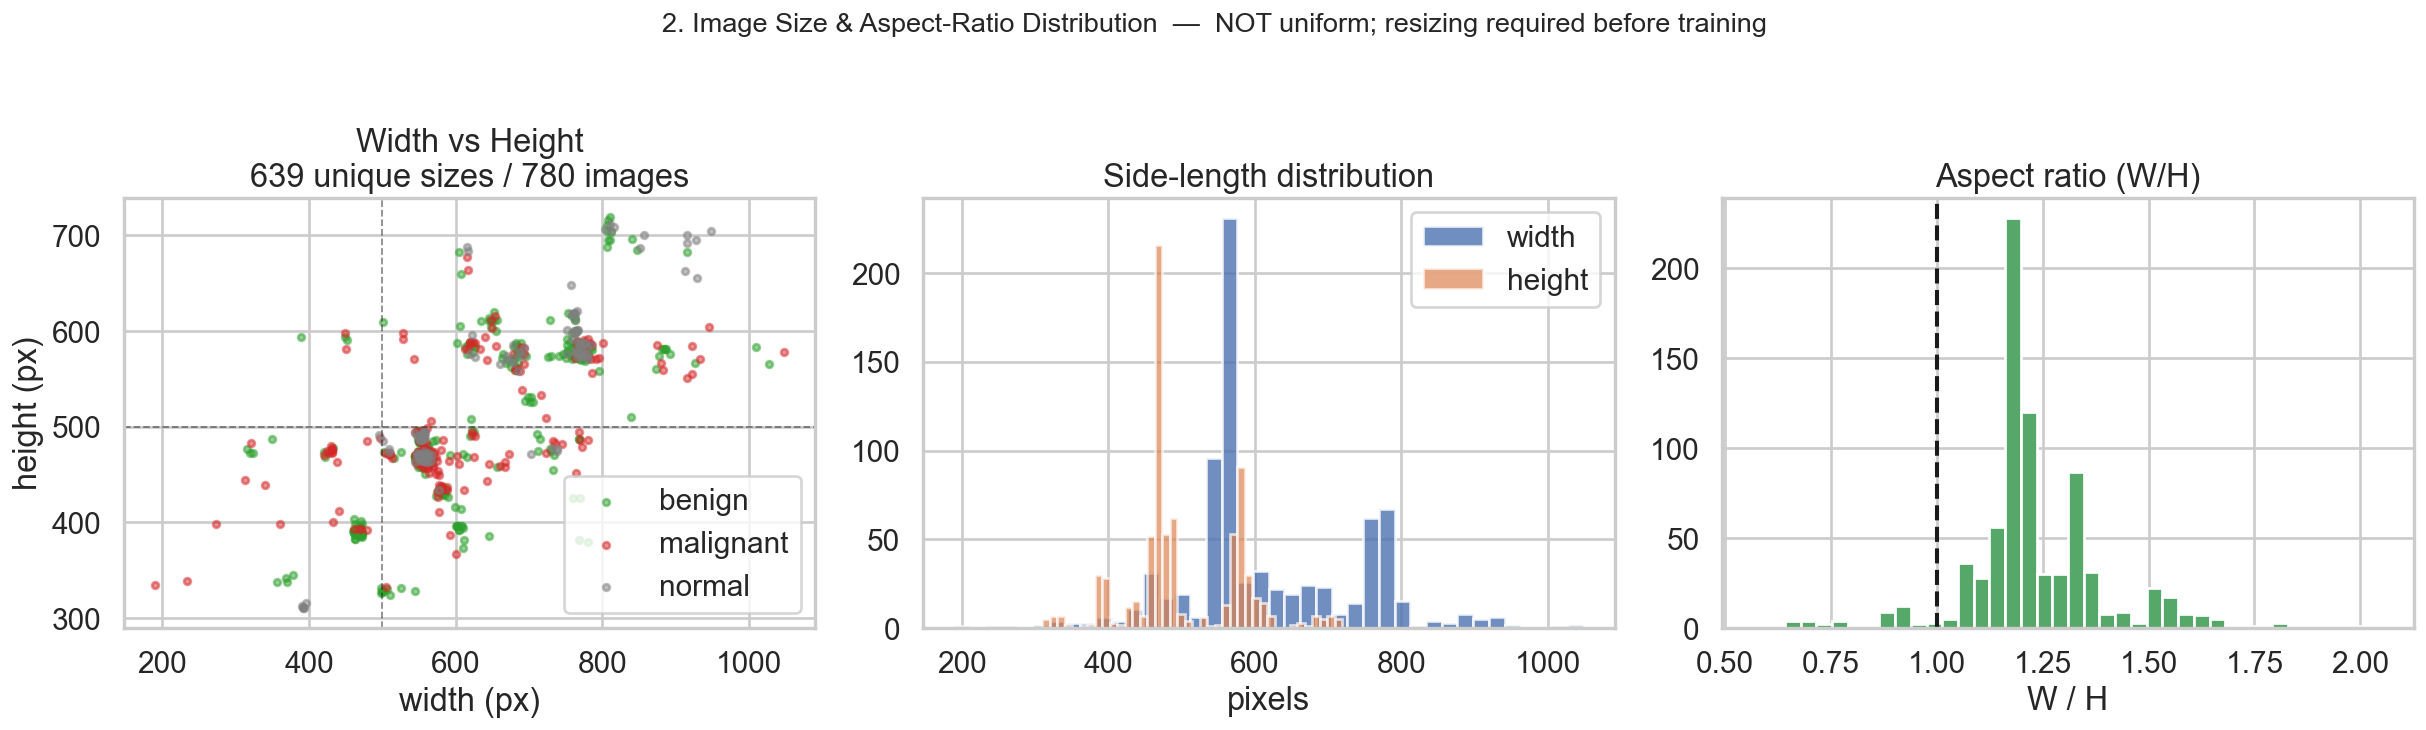
\includegraphics[width=\linewidth]{fig02_image_size}
  \caption{Image dimensions / aspect ratio.}
  \label{fig:imgsize}
\end{subfigure}\hfill
\begin{subfigure}{0.49\linewidth}
  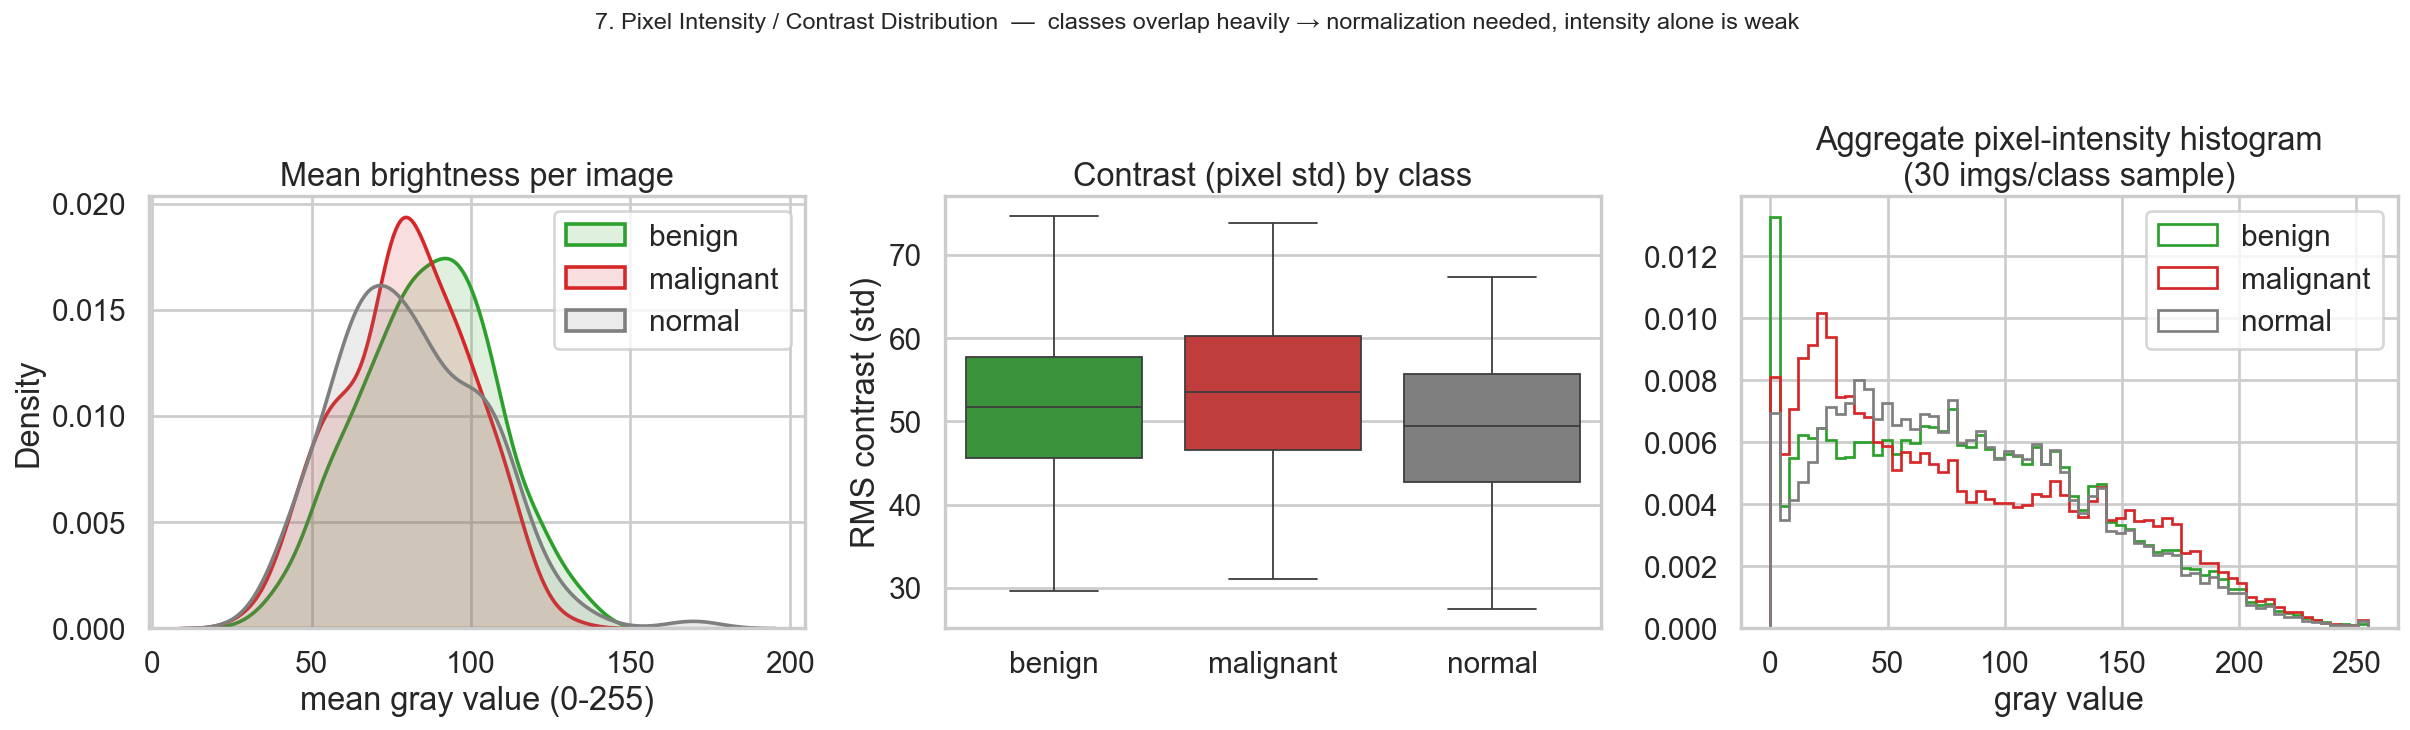
\includegraphics[width=\linewidth]{fig07_intensity}
  \caption{Per-class pixel-intensity / contrast.}
  \label{fig:intensity}
\end{subfigure}
\caption{Image properties. (a)~Sizes are inconsistent and mostly landscape,
motivating letterbox resizing to a fixed $256\times256$. (b)~Brightness and
contrast overlap across classes, so intensity alone is a weak feature and
per-image normalisation is used.}
\label{fig:imgprops}
\end{figure}

\subsection{Lesion size, location and morphology}
\label{sec:eda-shape}
The masks let us quantify lesion geometry. The lesion-area ratio (lesion pixels
$\div$ image pixels) is much larger for malignant lesions (median $\approx 12\%$)
than for benign lesions (median $\approx 4\%$) (Fig.~\ref{fig:area}). This has two
consequences: lesion \emph{size is itself discriminative}, and many benign lesions
are \emph{very small}, creating a strong pixel-level foreground/background
imbalance that favours an overlap-aware segmentation loss (Dice/Tversky rather
than pixel accuracy). Aligned per-class mask heatmaps show that lesions
concentrate \emph{near the image centre, slightly above the middle}
(Fig.~\ref{fig:location}), an acquisition bias arising because sonographers centre
the probe on the finding; random crops/translations during training reduce
over-reliance on this position cue. Finally, shape descriptors computed from the
masks (circularity, solidity, extent, bounding-box aspect and eccentricity) show
that malignant lesions have \emph{lower circularity, solidity and extent and
higher eccentricity} than benign lesions (Fig.~\ref{fig:shape}), quantifying their
``irregular, spiculated'' appearance. These shape differences later motivate two
things: boundary-aware/attention segmentation models, and the shape/radiomics
feature-fusion experiment in the dual-stage classifier (Section~\ref{sec:improved-dual}).

\begin{figure}[t]
\centering
\begin{subfigure}{0.49\linewidth}
  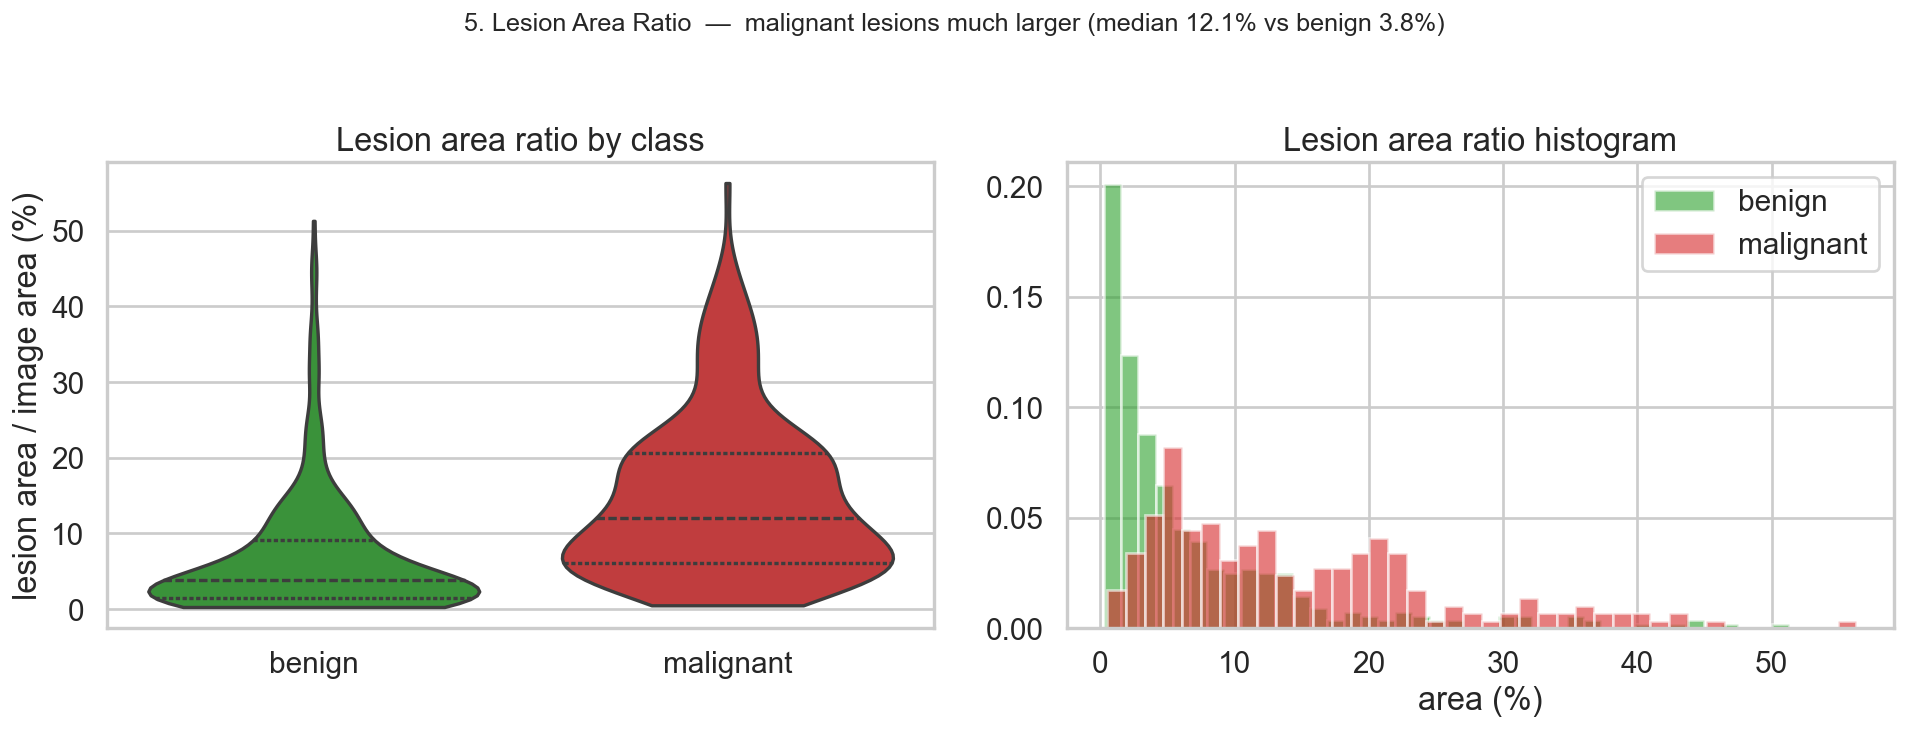
\includegraphics[width=\linewidth]{fig05_area_ratio}
  \caption{Lesion-area ratio by class.}
  \label{fig:area}
\end{subfigure}\hfill
\begin{subfigure}{0.49\linewidth}
  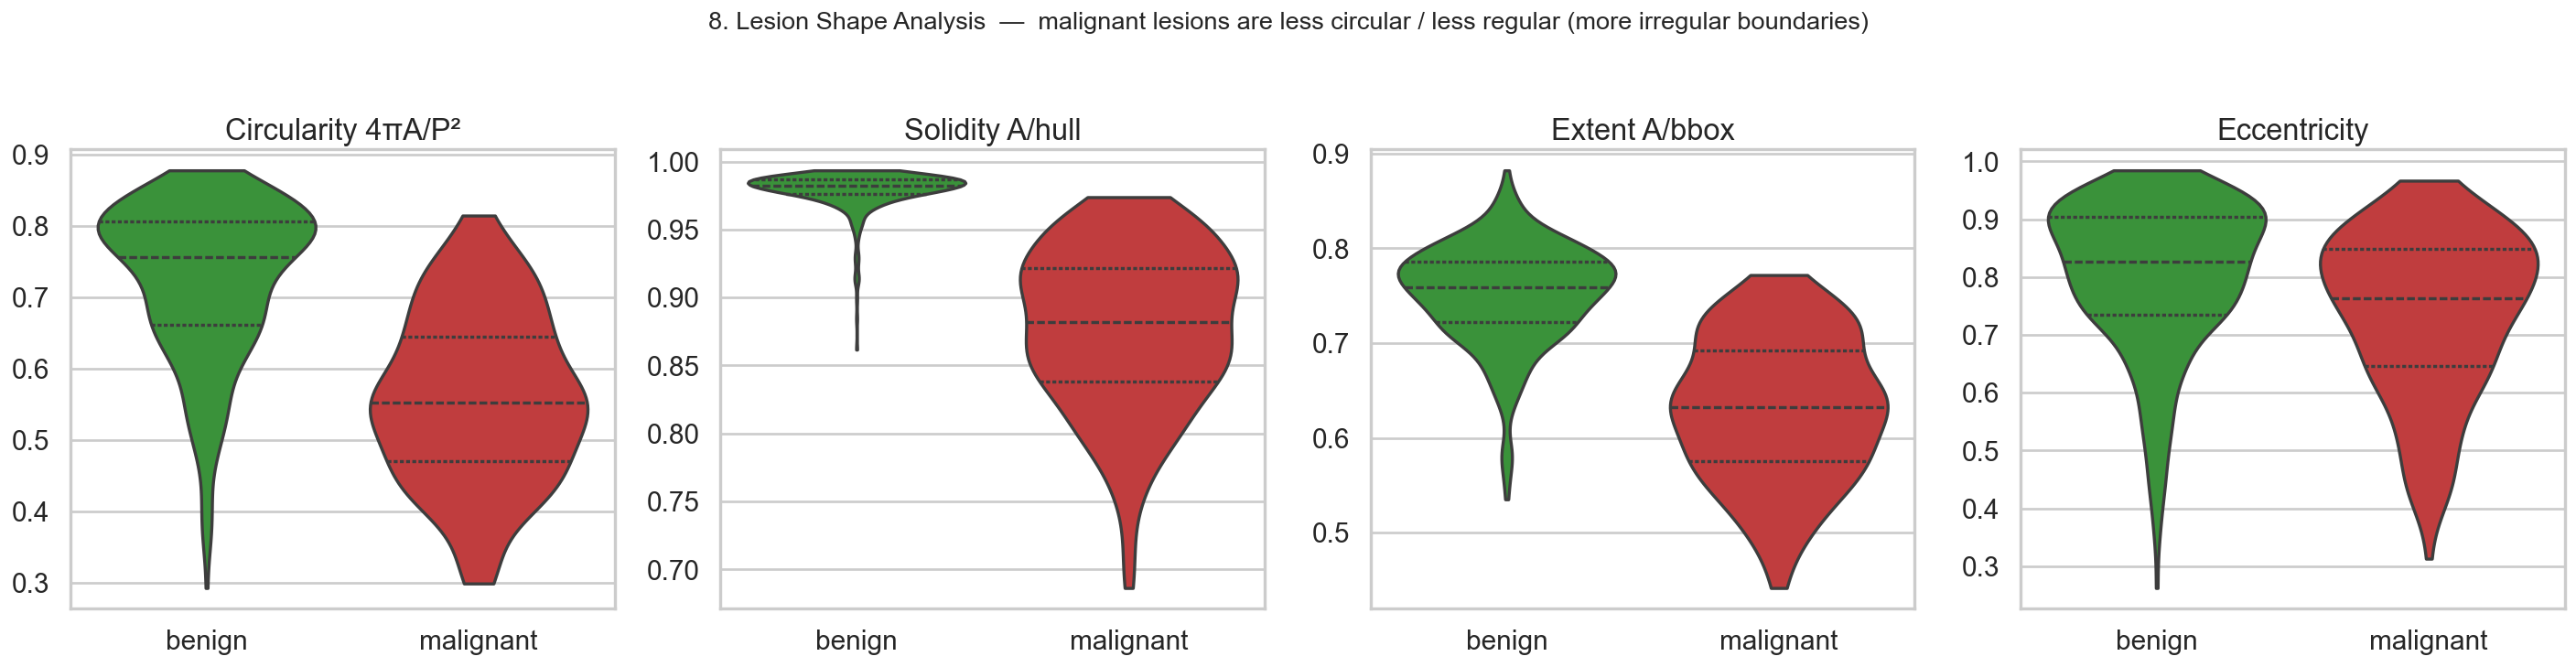
\includegraphics[width=\linewidth]{fig08_shape}
  \caption{Lesion shape descriptors by class.}
  \label{fig:shape}
\end{subfigure}
\caption{Lesion morphology. (a)~Malignant lesions are larger (median
$\approx 12\%$ vs.\ $\approx 4\%$ of the image); many benign lesions are tiny.
(b)~Malignant lesions are less circular/solid and more eccentric, i.e.\ more
irregular. Both findings inform loss choice, model choice and the shape-feature
experiment.}
\label{fig:morph}
\end{figure}

\begin{figure}[t]
\centering
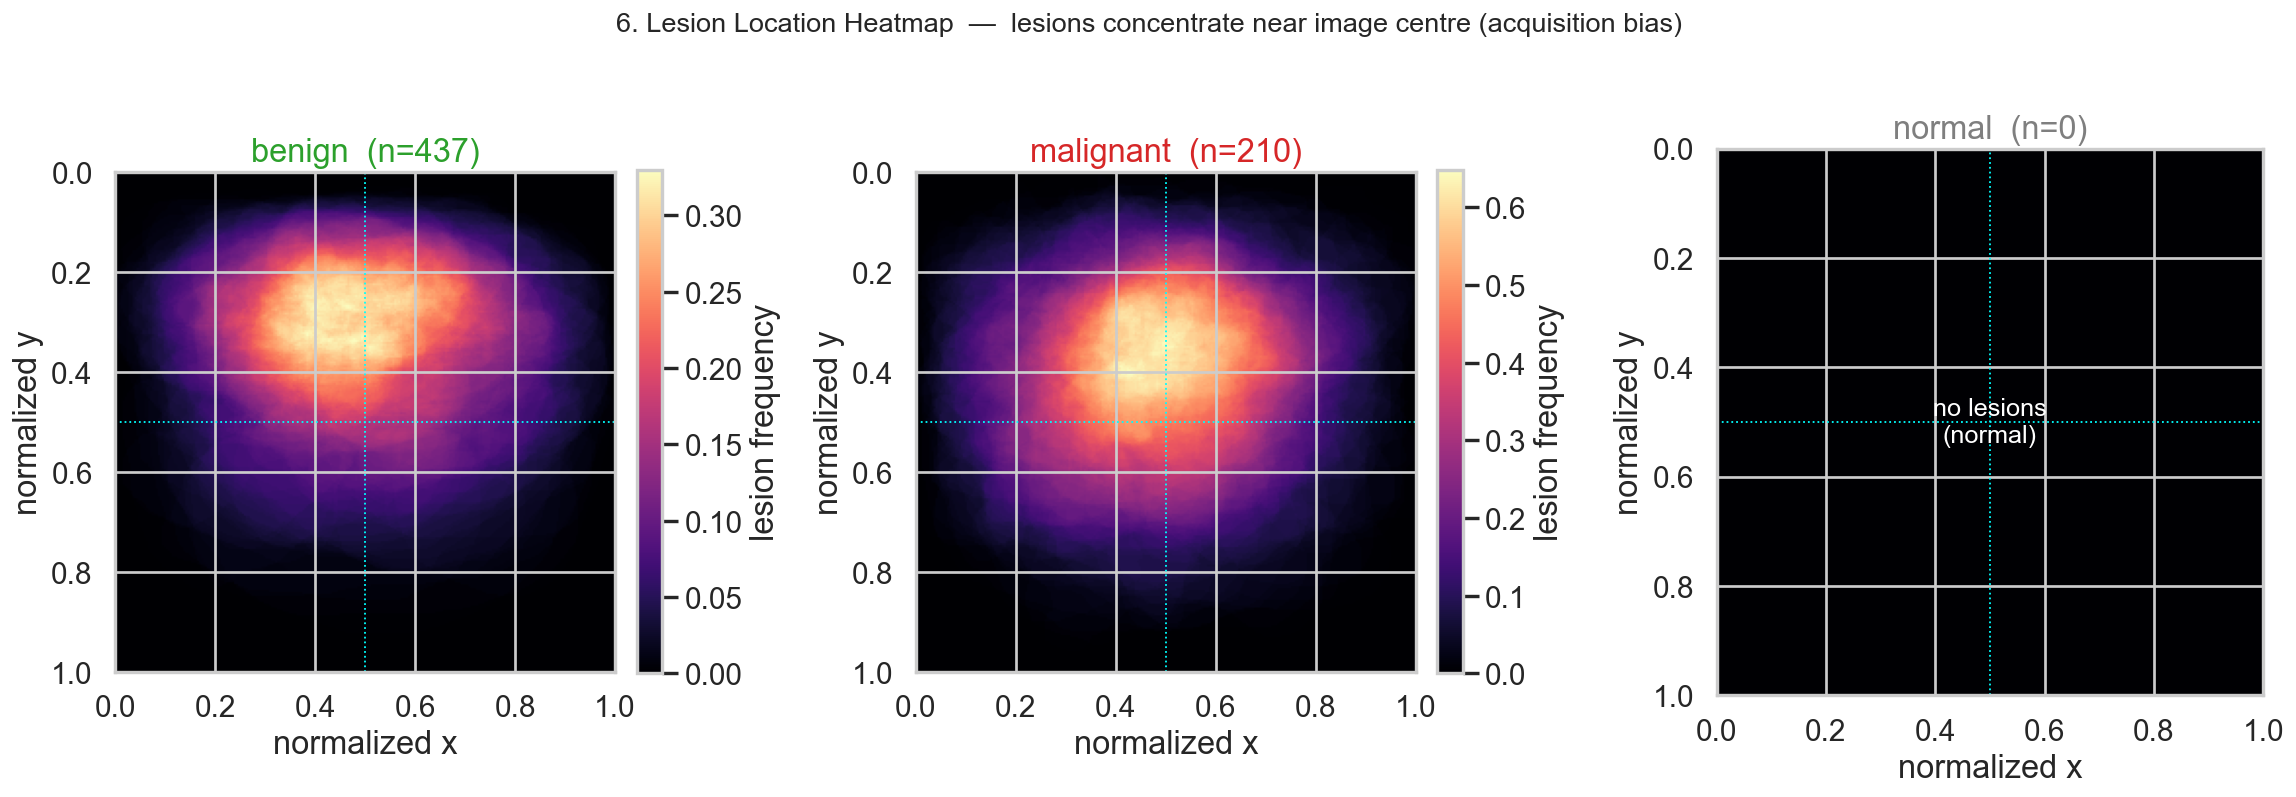
\includegraphics[width=0.9\linewidth]{fig06_location_heatmap}
\caption{Aligned per-class lesion-location heatmaps. Lesions concentrate near the
image centre (an acquisition bias); \texttt{normal} has no lesion signal. This
motivates translation/crop augmentation so the model does not simply exploit
lesion position.}
\label{fig:location}
\end{figure}

\subsection{Duplicate images, label conflicts and leakage risk}
\label{sec:eda-dup}
This is the most consequential integrity check. We detect \emph{exact}
duplicates via MD5 hashing of file bytes and \emph{near}-duplicates via a
perceptual hash (pHash) with Hamming distance. We find an \textbf{exact
cross-class duplicate}: \texttt{benign (433).png} and \texttt{malignant
(145).png} are the same file bytes but carry \emph{different} class labels -- a
genuine labelling conflict. More broadly, at a Hamming threshold of $5$ there are
$186$ near-duplicate pairs, of which $10$ \emph{cross class boundaries}; these
group into $124$ clusters covering $277$ images ($36\%$ of the data)
(Fig.~\ref{fig:dup}). This is consistent with a documented BUSI data-quality
issue~\cite{pawlowska2023}.

Near-duplicates are dangerous for evaluation. Simulating naive random $70/30$
image-level splits, on the order of $57$ near-duplicate clusters end up with
copies on \emph{both} the train and test sides (Fig.~\ref{fig:leakage}); the test
set then contains images the model effectively saw in training, which inflates
the reported accuracy and Dice. Our remedy is threefold: drop the conflicting
exact duplicate, merge multi-masks by union, and split at the \emph{cluster}
level so that all near-duplicates of an image stay on a single side, while
stratifying by class. Table~\ref{tab:cleaning} summarises the cleaning and
grouping. This single decision is the main reason our reproductions score below
their published values (Section~\ref{sec:results}).

\begin{figure}[t]
\centering
\begin{subfigure}{0.52\linewidth}
  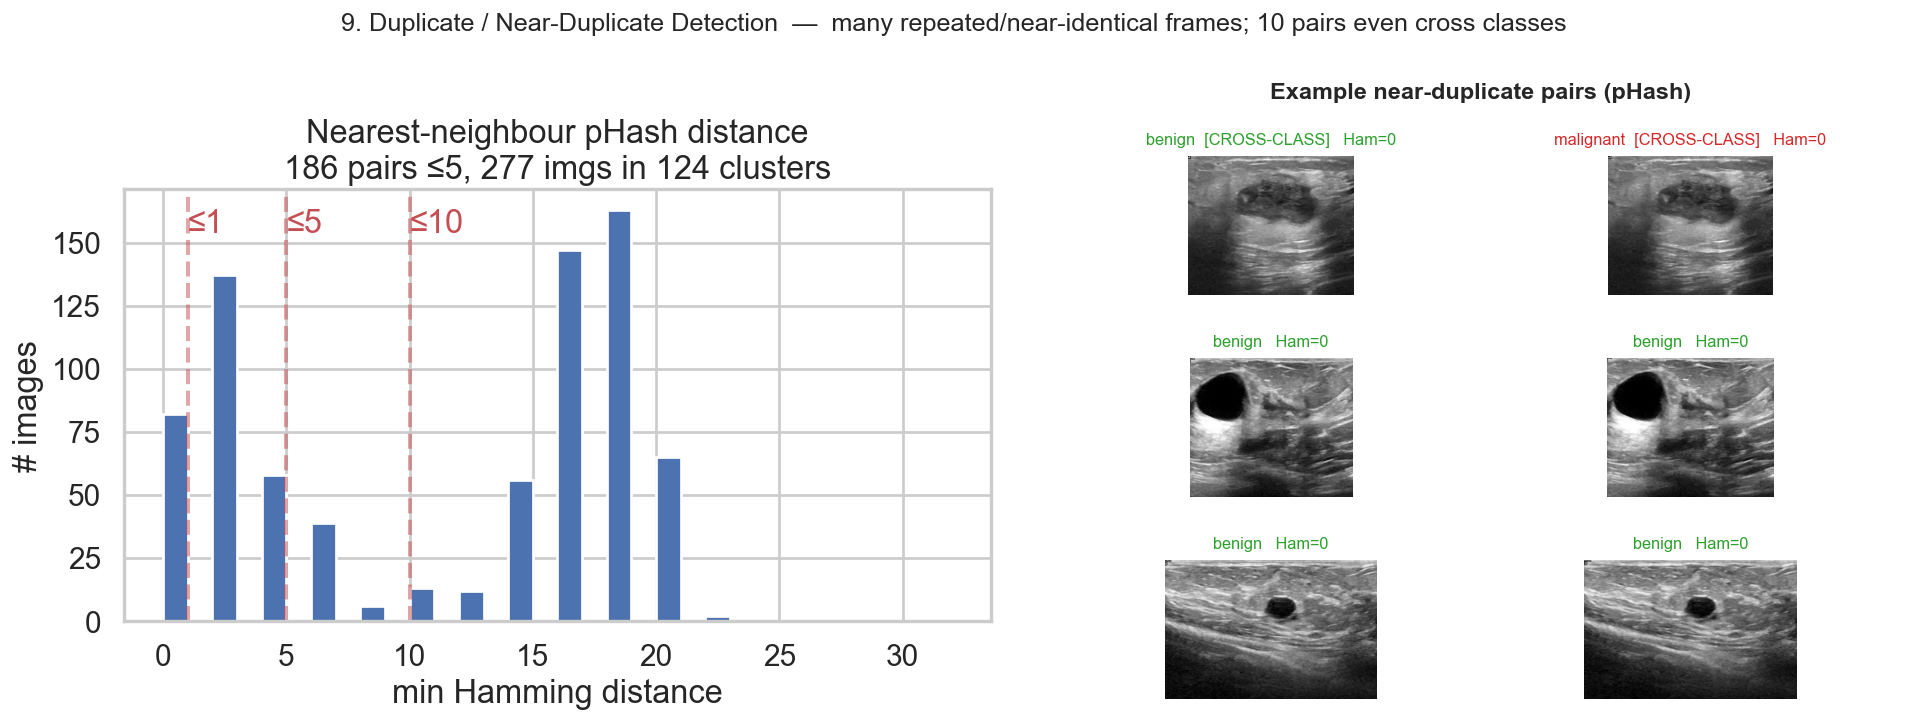
\includegraphics[width=\linewidth]{fig09_duplicates}
  \caption{Near-duplicate detection (pHash).}
  \label{fig:dup}
\end{subfigure}\hfill
\begin{subfigure}{0.46\linewidth}
  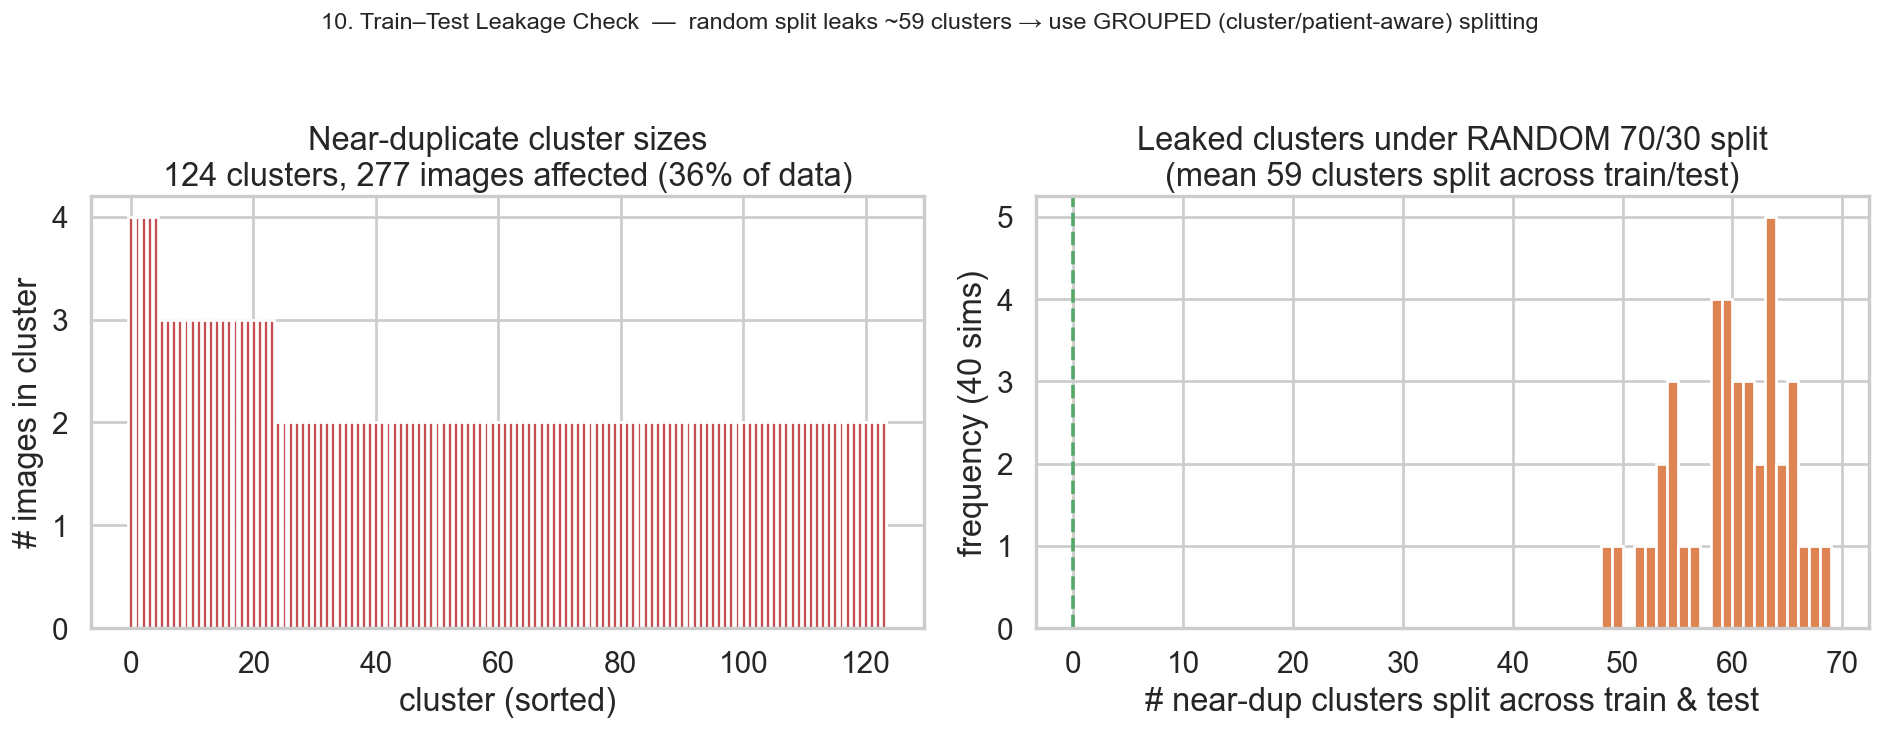
\includegraphics[width=\linewidth]{fig10_leakage}
  \caption{Leakage under random splitting.}
  \label{fig:leakage}
\end{subfigure}
\caption{Data-quality analysis. (a)~$186$ near-duplicate pairs ($10$ cross-class)
form $124$ clusters covering $36\%$ of BUSI, including an exact cross-class
duplicate. (b)~Simulated random $70/30$ splits leak dozens of clusters across
train/test (mean on the order of tens of clusters), motivating a cluster-grouped
split. Panel~(b) shows one $40$-run simulation.}
\label{fig:quality}
\end{figure}

\begin{table}[t]
\centering
\caption{Cleaning and grouping summary (from the notebook's data-quality
analysis).}
\label{tab:cleaning}
\small
\begin{tabular}{@{}lc@{}}
\toprule
Step & Value \\
\midrule
Exact-duplicate file pairs (MD5)                 & $1$ (cross-class conflict) \\
Near-duplicate pairs (pHash Hamming $\leq 5$)    & $186$ \\
\quad of which cross-class                       & $10$ \\
Near-duplicate clusters                          & $124$ \\
Images inside a cluster                          & $277$ ($36\%$ of data) \\
Clusters leaked by a naive random $70/30$ split  & $\approx 57$ (simulated) \\
Mitigation                                       & drop conflict; union masks; cluster-grouped stratified split \\
\bottomrule
\end{tabular}
\end{table}

\subsection{Pre-processing decisions}
\label{sec:eda-pre}
Every pre-processing choice is tied to an EDA observation rather than adopted by
default (Table~\ref{tab:preproc}). We \emph{resize with padding} (letterbox) to
$256\times256$ to preserve lesion aspect ratio; convert to grayscale for
from-scratch models or replicate to three ImageNet-normalised channels for
pretrained backbones; and normalise per image. On the training split only we
apply light augmentation (horizontal flips, small affine transforms and
brightness/contrast jitter), which addresses the small, imbalanced dataset and the
lesion-centre bias. Contrast-limited adaptive histogram equalisation (CLAHE) and
speckle denoising were considered but \emph{not} adopted in the shared pipeline:
BUSI images are low-contrast, but speckle is informative texture and aggressive
enhancement or denoising can distort it, so we treat these as optional steps to be
justified by an ablation rather than used blindly. We ran no dedicated
CLAHE/denoising ablation within the compute budget, so we state this as a
deliberate omission rather than as evidence that the two steps are useless; it is
listed in future work (Section~\ref{sec:future}).

\begin{table}[t]
\centering
\caption{Pre-processing decisions and their EDA justification.}
\label{tab:preproc}
\small
\begin{tabularx}{\linewidth}{@{}L{4.3cm} l Y@{}}
\toprule
Step & Decision & Justification (EDA) \\
\midrule
Resize to $256\times256$        & required  & Inconsistent sizes (\S\ref{sec:eda-img}); fixed input needed. \\
Letterbox (pad, keep ratio)     & preferred & Mostly landscape; naive resize distorts discriminative lesion shape (\S\ref{sec:eda-shape}). \\
Normalisation (per-image/ImageNet)& required & Wide, overlapping brightness (\S\ref{sec:eda-img}); stabilises training. \\
Grayscale vs.\ 3-channel        & model-dependent & Pseudo-RGB storage; 1 channel saves compute, 3 channels reuse ImageNet weights. \\
Augmentation (flip/affine/jitter)& training only & Small, imbalanced data + centre bias (\S\ref{sec:eda-imb},\ref{sec:eda-shape}). \\
CLAHE / denoising               & not adopted & Low contrast but informative speckle; risk of distortion -- ablation only. \\
De-duplicate + cluster split    & critical  & Duplicates and leakage (\S\ref{sec:eda-dup}) would inflate metrics. \\
\bottomrule
\end{tabularx}
\end{table}

\subsection{EDA implications for model design}
\label{sec:eda-implications}
Table~\ref{tab:implications} maps each headline EDA finding to a modelling
decision. These decisions carry directly into Sections~\ref{sec:models}
and~\ref{sec:setup}.

\begin{table}[H]
\centering
\caption{From EDA observation to modelling implication.}
\label{tab:implications}
\small
\begin{tabularx}{\linewidth}{@{}L{5.2cm} Y@{}}
\toprule
EDA observation & Modelling implication \\
\midrule
Small dataset overall                    & Transfer learning + augmentation + regularisation. \\
Class imbalance                          & Stratified split, class-weighted loss, macro-F1 + AUC. \\
Many tiny benign lesions                 & Overlap-aware loss (Dice/Tversky); report Dice/IoU; analyse recall. \\
Irregular malignant boundaries           & Attention / multi-scale segmentation models. \\
Near-duplicates                          & Cluster-grouped, leakage-free split. \\
Benign vs.\ malignant shape differences  & Evaluate shape/radiomics features in the classifier. \\
Lesion-centre acquisition bias           & Random crop/translation augmentation. \\
Overlapping intensity                    & Per-image normalisation; rely on texture/shape. \\
\bottomrule
\end{tabularx}
\end{table}

% =============================================================================
\section{Models and Methods}
\label{sec:models}
% =============================================================================
We reproduce thirteen published models and build two of our own. All models share
the same cleaned, cluster-grouped, leakage-free split, letterbox pre-processing
and metrics from \texttt{Models/common/}, so differences in the numbers reflect
the architecture and training recipe, not data handling. Table~\ref{tab:modeloverview}
gives an overview; we then describe each model consistently, noting which parts
are pretrained and which are our own implementation. For each model we
implemented the head/decoder and the training/evaluation loop ourselves;
pretrained backbones are reused torchvision or \texttt{segmentation-models-pytorch}
(smp) components, as indicated.

\begin{table}[t]
\centering
\caption{Overview of all models. ``Origin'': R\,=\,reproduced published model,
P\,=\,proposed by us. ``Backbone'': pretrained (PT) or from scratch (FS).
Parameter counts are read from the result files.}
\label{tab:modeloverview}
\scriptsize
\begin{tabularx}{\linewidth}{@{}l l L{3.0cm} c L{2.5cm} c c@{}}
\toprule
Model & Task & Backbone / main idea & PT/FS & Loss & Params (M) & Origin \\
\midrule
U-Net~\cite{ronneberger2015unet}            & Seg & encoder--decoder + skips        & FS & Dice+BCE       & $31.04$ & R \\
Attention U-Net~\cite{oktay2018attentionunet}& Seg & U-Net + attention gates         & FS & Dice+BCE       & $31.39$ & R \\
FCN-AlexNet~\cite{yap2018cnn}               & Seg & AlexNet $\to$ fully conv.       & PT & Dice+BCE       & $28.70$ & R \\
Patch-LeNet~\cite{yap2018cnn}               & Det & 28$\times$28 patch classifier   & FS & CE (patches)   & $0.43$  & R \\
DeepLabV3+~\cite{chen2018deeplabv3plus}     & Seg & ResNet-50 + ASPP                & PT & BCE+soft-Dice  & $26.69$ & R \\
nnU-Net~\cite{isensee2021nnunet}            & Seg & blueprint 2D U-Net + deep sup.  & FS & CE+Dice (DS)   & $8.55$  & R \\
AAU-Net~\cite{chen2023aaunet}               & Seg & hybrid adaptive attention       & FS & Dice+BCE       & $42.75$ & R \\
CResU-Net~\cite{derakhshandeh2024cresunet}  & Seg & Co-Block/residual schedule      & FS & Dice           & $33.54$ & R \\
ResNet-18~\cite{he2016resnet}               & Cls & residual backbone               & PT & weighted CE    & $11.18$ & R \\
DenseNet-121~\cite{huang2017densenet}       & Cls & dense connectivity              & PT & weighted CE    & n/r     & R \\
EfficientNet-B0~\cite{tan2019efficientnet}  & Cls & compound-scaled MBConv          & PT & weighted CE    & n/r     & R \\
Dual-stage~\cite{bruno2025dualstage}        & Both& DeepLabV3+ $\to$ ROI $\to$ EffB0& PT & weighted CE    & --      & R \\
MTL-OCA~\cite{lu2025multitask}              & Both& shared Res-UNet + OCA + cls     & FS & $0.4$CE$_s$+CE+CE& $8.19$ & R \\
\textbf{Improved U-Net (ours)}              & Seg & U-Net + \textbf{PT EffB4} enc.  & PT & Focal-Tversky+BCE& $20.23$ & \textbf{P} \\
\textbf{Improved dual-stage (ours)}         & Both& \textbf{Improved-UNet} $\to$ ROI $\to$ EffB0 & PT & weighted CE & -- & \textbf{P} \\
\bottomrule
\end{tabularx}
\end{table}

\subsection{Loss functions and metrics}
\label{sec:losses}
Let $p_i\in[0,1]$ be a predicted (foreground) probability and $g_i\in\{0,1\}$ the
ground truth over $N$ pixels (segmentation) or examples (classification).

\paragraph{Binary cross-entropy (BCE).}
\begin{equation}
\mathcal{L}_{\mathrm{BCE}} = -\frac{1}{N}\sum_{i=1}^{N}\Big[g_i\log p_i + (1-g_i)\log(1-p_i)\Big].
\end{equation}

\paragraph{Weighted multi-class cross-entropy.}
For $C$ classes with softmax output $p_{i,c}$ and one-hot label $g_{i,c}$,
\begin{equation}
\mathcal{L}_{\mathrm{wCE}} = -\frac{1}{N}\sum_{i=1}^{N}\sum_{c=1}^{C} w_c\, g_{i,c}\log p_{i,c},
\qquad w_c \propto \frac{N}{C\,n_c},
\end{equation}
where $n_c$ is the number of training examples of class $c$; the
\emph{inverse-frequency} weights $w_c$ counter the imbalance of
Section~\ref{sec:eda-imb}.

\paragraph{Dice coefficient and Dice loss.}
The Dice similarity coefficient (DSC) and its soft loss are
\begin{equation}
\mathrm{DSC} = \frac{2\sum_i p_i g_i + \epsilon}{\sum_i p_i + \sum_i g_i + \epsilon},
\qquad
\mathcal{L}_{\mathrm{Dice}} = 1-\mathrm{DSC},
\end{equation}
with $\epsilon$ a small constant for numerical stability. DSC emphasises overlap
and is well suited to the small-lesion foreground/background imbalance of
Section~\ref{sec:eda-shape}.

\paragraph{Intersection-over-Union (IoU/Jaccard).}
\begin{equation}
\mathrm{IoU} = \frac{|P\cap G|}{|P\cup G|} = \frac{\sum_i p_i g_i}{\sum_i p_i + \sum_i g_i - \sum_i p_i g_i}.
\end{equation}

\paragraph{Tversky index and Focal-Tversky loss.}
The Tversky index generalises Dice by weighting false positives (FP) and false
negatives (FN) asymmetrically:
\begin{equation}
T = \frac{\sum_i p_i g_i}{\sum_i p_i g_i + \alpha\sum_i p_i(1-g_i) + \beta\sum_i (1-p_i)g_i},
\end{equation}
and the Focal-Tversky loss~\cite{salehi2017tversky,abraham2019focaltversky} adds a
focusing exponent $\gamma$:
\begin{equation}
\mathcal{L}_{\mathrm{FT}} = (1-T)^{\gamma}.
\end{equation}
Choosing $\beta>\alpha$ penalises false negatives (missed lesion pixels) more
heavily, targeting the missed-lesion tail identified in
Section~\ref{sec:eda-shape}. Setting $\alpha=\beta=0.5,\ \gamma=1$ recovers the
Dice loss exactly, so Focal-Tversky is a strict generalisation and the ablation of
Section~\ref{sec:results-seg} is a controlled one.

\paragraph{Our combined segmentation loss.}
The improved segmenter is trained with a convex blend of BCE and Focal-Tversky,
\begin{equation}
\mathcal{L}_{\mathrm{combo}} = \lambda\,\mathcal{L}_{\mathrm{BCE}} +
(1-\lambda)\,\mathcal{L}_{\mathrm{FT}},
\qquad
\lambda = 0.5,\ \ \alpha = 0.3,\ \ \beta = 0.7,\ \ \gamma = \tfrac{4}{3},
\label{eq:combo}
\end{equation}
with the Tversky smoothing constant $\epsilon = 1$ and the index computed
\emph{per image} before averaging over the batch (so a large lesion cannot dominate
a small one). The values $(\alpha,\beta,\gamma)=(0.3,0.7,4/3)$ are the defaults
recommended by Abraham and Khan~\cite{abraham2019focaltversky} and were
\emph{not} tuned on our data, which keeps the ablation honest. The BCE term keeps
pixel-level gradients healthy early in training, when the Tversky term is nearly
flat; the Focal-Tversky term then drives the overlap metric and the false-negative
penalty. The identical loss (same $\lambda,\alpha,\beta,\gamma$) is used to
generate the out-of-fold training masks of Section~\ref{sec:improved-dual}.

\paragraph{Classification metrics.}
With per-class precision $P_c$ and recall $R_c$, the class F1 and macro-F1 are
\begin{equation}
\mathrm{F1}_c = \frac{2P_cR_c}{P_c+R_c},\qquad
\text{macro-F1} = \frac{1}{C}\sum_{c=1}^{C}\mathrm{F1}_c .
\end{equation}
Macro-F1 weights every class equally and is our primary classification metric
(Section~\ref{sec:eval}); we also report balanced accuracy, accuracy, macro
one-vs-rest ROC-AUC and the confusion matrix. Segmentation is scored with
\emph{per-image} Dice and IoU (averaged over images, so large lesions do not
dominate), pixel precision/recall, and the Yap detection metrics
(true-positive fraction, false positives per image, F-measure) where
applicable~\cite{yap2018cnn}.

\subsection{Reproduction: the project's three required papers}
\label{sec:repro3}
The brief names three papers -- the BUSI dataset~\cite{aldhabyani2020busi}, Yap et
al.~\cite{yap2018cnn} and U-Net~\cite{ronneberger2015unet} -- so we first
reproduce the three models these define.

\textbf{U-Net (from scratch)~\cite{ronneberger2015unet}.} A four-level
contracting/expanding encoder--decoder of double $3\times3$ convolutions with
$2\times2$ pooling and skip connections that concatenate encoder features into the
decoder; we pad convolutions to preserve size, add batch normalisation, and output
a single-channel logit map from a $1\times256\times256$ grayscale input, trained
with Dice+BCE. \emph{Own work:} the whole architecture and training loop. It is
our from-scratch segmentation reference and the baseline of the improved-segmenter
ablation.

\textbf{Patch-based LeNet (detection)~\cite{yap2018cnn}.} A small LeNet classifies
$28\times28$ grayscale patches as lesion vs.\ non-lesion; at test time a sliding
window builds a lesion-probability map that is thresholded into a detection map.
We train it with balanced hard-negative sampling. This is a \emph{detection}
method, scored with the Yap detection metrics. \emph{Own work:} the LeNet, the
balanced/hard-negative patch sampler and the sliding-window inference.

\textbf{FCN-AlexNet (Yap's best method)~\cite{yap2018cnn}.} An ImageNet-pretrained
AlexNet is made fully convolutional (fc6/fc7 recast as convolutions, a $1\times1$
score convolution and bilinear upsampling) and fine-tuned for segmentation.
\emph{Own work:} the fully convolutional head and fine-tuning; the AlexNet
backbone is a pretrained component.

\subsection{Additional segmentation models}
\label{sec:repro-seg}
\textbf{Attention U-Net~\cite{oktay2018attentionunet}} augments our U-Net with an
additive attention gate on every skip connection, computing an attention map
$\alpha=\sigma(\psi\,\mathrm{ReLU}(W_x x + W_g g))$ and re-weighting the skip as
$\alpha x$. It uses the \emph{same} loss and recipe as our U-Net, so it is a
controlled test of the attention gate. \emph{Own work:} the attention-gate module.
\textbf{DeepLabV3+~\cite{chen2018deeplabv3plus}} uses an ImageNet-pretrained
ResNet-50 encoder (output stride $16$) feeding an ASPP head and a light decoder;
it is our strongest \emph{reproduced} segmenter. \emph{Own work:} the ASPP head and
decoder; the ResNet-50 is pretrained. \textbf{nnU-Net~\cite{isensee2021nnunet}} is
reproduced as its fixed \emph{blueprint} 2D U-Net (Conv--InstanceNorm--LeakyReLU,
strided-conv down, transposed-conv up, deep supervision), trained with the nnU-Net
recipe; we deliberately drop the self-configuring framework, so this is an
architecture-and-recipe reproduction. \emph{Own work:} the network,
deep-supervision loss and loop. \textbf{AAU-Net~\cite{chen2023aaunet}} reproduces
the Hybrid Adaptive Attention Module (multi-receptive-field convolutions with
channel and spatial self-attention); \emph{own work:} the HAAM module and network,
written from scratch. \textbf{CResU-Net~\cite{derakhshandeh2024cresunet}} schedules
Co-Block (dense-concatenation), ResNet-identity and MultiRes encoder blocks and is
trained with a pure Dice loss (paper-faithful); \emph{own work:} the three block
types and the block-scheduled U-Net.

\subsection{Classification models}
\label{sec:repro-cls}
All three backbones take a three-channel ImageNet-normalised $256\times256$ input
(grayscale replicated to pseudo-RGB), have their final layer replaced by a fresh
three-way head, and are fine-tuned with inverse-frequency weighted cross-entropy.
We deliberately use the \emph{smallest} variant of each family because BUSI is
small. \textbf{ResNet-18~\cite{he2016resnet}} is fine-tuned with SGD;
\textbf{DenseNet-121~\cite{huang2017densenet}} adds dropout before the head and is
trained with early stopping on validation macro-F1;
\textbf{EfficientNet-B0~\cite{tan2019efficientnet}} adds dropout before a
three-way head. \emph{Own work:} the heads and training pipelines.

\subsection{Combined segmentation--classification}
\label{sec:combined}
\textbf{Dual-stage pipeline (reproduced)~\cite{bruno2025dualstage}.} Stage-1
DeepLabV3+ predicts the lesion mask; from the predicted mask we take the largest
connected component, expand its bounding box and crop the ROI (falling back to the
full frame if no lesion is found); Stage-2 is an EfficientNet-B0 with a fresh
two-way head trained on the ROI crops to classify benign vs.\ malignant. We follow
the paper's two-class setting and reuse our ResNet-50 DeepLabV3+ as Stage-1.
\emph{Own work:} the ROI coupling (mask $\to$ bounding box $\to$ crop) and the
end-to-end pipeline. The coupling is deterministic and is worth stating precisely,
because it is held \emph{fixed} across every dual-stage variant we compare: on the
binarised $256\times256$ mask we run 8-connected component labelling, keep the
component of largest area, take its axis-aligned bounding box $(x,y,w,h)$ and
dilate it by a relative margin of $15\%$ per side
($x_0=\max(0,x-0.15w)$, $x_1=\min(W,x+w+0.15w)$, and likewise in $y$), clipping to
the image. Boxes whose shorter side falls below $16$\,px are rejected as
unusable. If the box is rejected or the mask is empty, the \emph{whole frame} is
passed to Stage-2 -- the paper's behaviour, so that a missed segmentation still
produces a prediction rather than an abstention. The crop is finally resized to
$256\times256$ for Stage-2. We report both the full pipeline score (predicted-mask ROI)
and a \emph{ground-truth-ROI (GT-ROI) upper bound}, in which Stage-2 is fed
ground-truth-mask crops -- a diagnostic for perfect segmentation.
\textbf{Multi-task MTL-OCA (reproduced)~\cite{lu2025multitask}.} A shared Res-UNet
backbone feeds an Object Contextual Attention segmentation head and a
global-average-pooled MLP three-class head, trained with the combined loss
$\mathcal{L}=0.4\,\mathrm{CE}_{\text{soft}}+\mathrm{CE}_{\text{final}}+\mathrm{CE}_{\text{cls}}$.
The paper's ``OASBUD'' statistics match BUSI, so we reproduce it on BUSI.
\emph{Own work:} the Res-UNet, OCA head, classification head and multi-task loop.

\subsection{Our improved segmenter}
\label{sec:improved-seg}
Our improvement is framed as a hypothesis rather than a mere architecture: the
only reproduced segmenter that used transfer learning (DeepLabV3+) clearly
out-scored the from-scratch ones (Section~\ref{sec:results}), so we hypothesise
that \emph{transfer learning is the decisive factor} for BUSI segmentation. We
therefore build a U-Net whose \textbf{encoder is an ImageNet-pretrained
EfficientNet-B4} (via smp), keeping the U-Net decoder and skip structure. On top
of this we test two further ideas suggested by the EDA: a \textbf{Focal-Tversky +
BCE} loss (Eq.~\ref{eq:combo}) to attack the missed-lesion tail
(Section~\ref{sec:eda-shape}), and \textbf{test-time augmentation (TTA)}
(horizontal-flip and multi-scale) with \textbf{largest-connected-component
post-processing}.

The inference path is fully specified as follows, since two of the four ablation
rows differ only in it. TTA averages the sigmoid probability maps of the original
image, its horizontal flip (un-flipped again before averaging) and two rescaled
copies (resized, forwarded, resized back), so the network is queried four times per
image; averaging probabilities rather than binary masks avoids a hard vote on
uncertain pixels. The averaged map is thresholded at a fixed $0.5$, closed with an
elliptical $5\times5$ morphological \texttt{CLOSE} to seal small holes along fuzzy
boundaries, and reduced to its largest 8-connected component with components below
$30$\,px discarded. The single-lesion assumption behind that last step is
justified by the EDA: after union-merging, essentially every image carries one
lesion region (Section~\ref{sec:eda-comp}). We evaluate each ingredient in a controlled ablation whose
components are: (a) the from-scratch U-Net baseline; (b) $+$ pretrained EfficientNet-B4
encoder (loss still Dice+BCE); (c) $+$ Focal-Tversky loss; (d) $+$
TTA+post-processing (the full model). \emph{Own work:} the model assembly, loss,
TTA/post-processing and the ablation.

\subsection{Our improved dual-stage pipeline}
\label{sec:improved-dual}
Starting from the reproduced dual-stage pipeline we make three changes and then
evaluate them rigorously.
\emph{(i) Stronger Stage-1 (controlled substitution).} We replace Stage-1 with our
improved segmenter and keep the ROI coupling and the Stage-2 classifier
\emph{byte-for-byte identical}, so any change in the end-to-end score is
attributable to segmentation alone.
\emph{(ii) Strengthened Stage-2.} The original pipeline trains Stage-2 on clean
ground-truth-mask ROI crops but tests it on imperfect predicted-mask crops, a
train/test distribution mismatch. We instead train Stage-2 on \emph{both}
ground-truth and predicted-mask ROI crops, select on predicted-ROI validation
macro-F1, and add horizontal-flip TTA.
\emph{(iii) Feature fusion.} From the predicted mask we optionally compute
\emph{shape} features ($6$ descriptors) or \emph{radiomics} features ($14$) and
concatenate them to the pooled EfficientNet-B0 embedding before the two-way head,
so the classifier sees deep features and explicit geometry together. The six shape
descriptors are exactly the EDA descriptors of Section~\ref{sec:eda-shape},
computed on the largest connected component of the predicted mask (all zero if the
mask is empty):
\begin{equation}
\text{area ratio} = \frac{A}{HW},\quad
\text{circularity} = \frac{4\pi A}{P^2},\quad
\text{solidity} = \frac{A}{A_{\mathrm{hull}}},\quad
\text{extent} = \frac{A}{wh},
\end{equation}
plus the bounding-box aspect $w/h$ and the eccentricity of the best-fit ellipse,
where $A$ and $P$ are the component's area and perimeter, $A_{\mathrm{hull}}$ its
convex-hull area and $(w,h)$ its bounding-box size. The $14$-D radiomics vector
extends these with $3$ intensity statistics (mean, standard deviation and median
grey level \emph{inside} the mask) and $5$ Haralick GLCM texture statistics
(contrast, dissimilarity, homogeneity, energy, correlation), computed on the
grey levels quantised to $32$ bins at offset $1$ and averaged over the
$0^{\circ}$ and $90^{\circ}$ directions; these are the classical BUS-CAD features
of the Cheng and Xian surveys~\cite{cheng2010survey,xian2018survey}. Crucially, the
features are computed from the \emph{predicted} mask at both training and test
time, so the classifier never sees geometry it would not have at deployment.

Crucially, we evaluate these candidate improvements rigorously. To train Stage-2
on predicted-mask crops we need predicted masks for the \emph{training} images; if
these came from a segmenter that had already seen those images the masks would be
unrealistically clean. We therefore generate them \emph{out-of-fold (OOF)} by
five-fold cross-fitting, so each training image's mask comes from a segmenter that
never saw it -- a correctness measure, not a way to raise the score. Every
configuration is run as a \emph{five-seed} ensemble and we report a bootstrap
$95\%$ confidence interval on the $98$-image test set. \emph{Own work:} the Stage-1
substitution, the strengthened/OOF Stage-2 protocol, the shape/radiomics fusion
and the multi-seed$+$CI evaluation.

\paragraph{On comparing the two headline numbers.}
The segmenter's Dice ($0.760$) and the pipeline's macro-F1 ($\approx 0.87$) measure
\emph{different tasks} on different test subsets and are not directly comparable. A
mask with Dice $0.76$ still localises the lesion well enough to crop a useful ROI;
the classifier then operates on the cropped pixels and does not need a
pixel-perfect boundary. Indeed the predicted-mask pipeline matches the GT-ROI
upper bound (Section~\ref{sec:results-dual}), confirming that segmentation quality
is not the bottleneck.

% =============================================================================
\section{Experimental Setup}
\label{sec:setup}
% =============================================================================
\subsection{Data split and leakage prevention}
\label{sec:setup-split}
All models use one cluster-grouped, class-stratified split
(Section~\ref{sec:eda-dup}), built once by \texttt{Models/\allowbreak common/\allowbreak data.py} and cached
to \texttt{split.csv} / \texttt{split\_cls.csv} so that every training script reads
the \emph{same} file. The procedure is: drop the exact cross-class duplicate pair,
union-merge multi-mask images, assign each image a near-duplicate cluster id
(pHash, Hamming $\leq 5$; singletons get their own id), then shuffle the
\emph{clusters} of each class with a fixed seed ($42$) and allocate whole clusters
to train/validation/test in $70/15/15$ proportion. Because the allocation is done
per class, the split is stratified; because it is done on clusters, no
near-duplicate can straddle the boundary.

The segmentation task uses the $645$ benign+malignant lesion images, split
$445/102/98$ (train/validation/test) over $532$ clusters; the three-class
classification task uses all $778$ retained images, split $540/120/118$ over $626$
clusters; the dual-stage pipeline is evaluated on the $98$-image two-class
(benign/malignant) test subset, which is by construction a subset of the $118$-image
three-class test set, so the two tasks are scored on consistent data.
Table~\ref{tab:split} gives the per-class composition. A programmatic sanity check
(\texttt{data.\_report\_split}) confirms that \emph{zero} clusters span more than
one split in either task -- the assertion that makes the whole benchmark
leakage-free. Note that the class proportions of each split match the global
$56/27/17$ ratio of Section~\ref{sec:eda-imb} to within about one percentage point,
so no split is accidentally easier than another. Augmentation is applied to the
training split \emph{only}; validation data is used for model selection (checkpoint
and threshold), and the test set is untouched during training and tuning.

\begin{table}[t]
\centering
\caption{Composition of the shared leakage-free split (from
\texttt{Models/common/split.csv} and \texttt{split\_cls.csv}). ``Clusters'' counts
near-duplicate clusters, the unit that is actually allocated; the last row is the
leakage assertion.}
\label{tab:split}
\small
\begin{tabular}{@{}l ccc c@{\hspace{2.2em}} cccc c@{}}
\toprule
& \multicolumn{4}{c}{Segmentation (2 classes, $645$ imgs)} & \multicolumn{5}{c}{Classification (3 classes, $778$ imgs)} \\
\cmidrule(lr){2-5}\cmidrule(lr){6-10}
Split & benign & malig. & total & clusters & normal & benign & malig. & total & clusters \\
\midrule
Train      & $298$ & $147$ & $445$ & --- & $95$ & $298$ & $147$ & $540$ & --- \\
Validation & $71$  & $31$  & $102$ & --- & $18$ & $71$  & $31$  & $120$ & --- \\
Test       & $67$  & $31$  & $98$  & --- & $20$ & $67$  & $31$  & $118$ & --- \\
\midrule
All        & $436$ & $209$ & $645$ & $532$ & $133$ & $436$ & $209$ & $778$ & $626$ \\
\multicolumn{10}{@{}l}{Clusters spanning $>1$ split: $\mathbf{0}$ (segmentation) \quad $\mathbf{0}$ (classification)} \\
\bottomrule
\end{tabular}
\end{table}

\subsection{Training configuration}
\label{sec:setup-train}
Table~\ref{tab:hparams} lists the training configuration of every model, read from
the result files. Settings differ between models because each follows its source
paper's recipe where practical; we did not force a single shared recipe, since
doing so would misrepresent the reproductions. What \emph{is} shared, and is what
makes the comparison fair, is everything upstream of the optimiser: the split, the
letterbox pre-processing, the augmentation policy of Table~\ref{tab:aug}, the
metric code and the test set.

\paragraph{Shared augmentation policy.}
Augmentation is implemented once in \texttt{Models/common/data.py} with
Albumentations and applied to the training split only. Its parameters are
deliberately conservative, because BUSI is small enough that aggressive
photometric distortion destroys the speckle texture the models rely on
(Section~\ref{sec:eda-pre}). For segmentation the geometric transforms are applied
jointly to the image and its mask so the pair stays registered; for classification
the same transforms are applied image-only. Table~\ref{tab:aug} lists the exact
settings and ties each to its EDA motivation. Note that we deliberately do
\emph{not} use vertical flips or large rotations: an ultrasound frame has a fixed
top-down geometry (probe surface at the top, depth increasing downwards), so a
vertical flip would produce an anatomically impossible image.

\begin{table}[t]
\centering
\caption{Shared training-time augmentation (\texttt{Models/common/data.py}).
Applied to the training split only; geometric transforms are applied jointly to
image and mask for segmentation.}
\label{tab:aug}
\small
\begin{tabularx}{\linewidth}{@{}l l Y@{}}
\toprule
Transform & Parameters & Motivation \\
\midrule
Horizontal flip        & $p=0.5$ & Left/right breast is arbitrary; doubles effective data. \\
Affine: scale          & $[0.9,\,1.1]$ & Lesion size varies with depth/probe setting (\S\ref{sec:eda-shape}). \\
Affine: translation    & $\pm5\%$ of side & Breaks the lesion-centre acquisition bias (\S\ref{sec:eda-shape}). \\
Affine: rotation       & $\pm15^{\circ}$ & Small probe-angle variation; larger angles are unphysical. \\
Brightness/contrast    & $\pm0.2$, $p=0.3$ & Wide inter-image brightness range (\S\ref{sec:eda-img}). \\
Vertical flip, elastic & \emph{not used} & Would violate the fixed top-down US geometry. \\
\bottomrule
\end{tabularx}
\end{table}

\begin{table}[t]
\centering
\caption{Training configuration per model (from the result JSON files). LR = initial
learning rate; wCE = inverse-frequency weighted cross-entropy; DS = deep
supervision. All inputs are $256\times256$.}
\label{tab:hparams}
\scriptsize
\begin{tabularx}{\linewidth}{@{}l c c l l l@{}}
\toprule
Model & Epochs & Batch & Optimiser (LR) & Scheduler & Loss \\
\midrule
U-Net                & $60$  & $8$  & Adam ($10^{-3}$)               & --           & Dice+BCE \\
Attention U-Net      & $60$  & $8$  & Adam ($10^{-3}$)               & --           & Dice+BCE \\
FCN-AlexNet          & $60$  & $8$  & SGD-m$0.9$ ($10^{-3}$)         & --           & Dice+BCE \\
Patch-LeNet          & $40$  & $256$& RMSprop ($10^{-2}$)            & --           & CE (patches) \\
DeepLabV3+           & $60$  & $8$  & AdamW$_{wd=10^{-4}}$ ($10^{-4}$)& cosine      & BCE+soft-Dice \\
nnU-Net              & $200$ & $8$  & SGD-Nesterov$0.99$ ($10^{-2}$) & poly$^{0.9}$ & CE+Dice (DS) \\
AAU-Net              & $80$  & $8$  & Adam ($10^{-3}$)               & cosine       & Dice+BCE \\
CResU-Net            & $120$ & $8$  & Adam ($10^{-3}$)               & cosine       & Dice \\
ResNet-18            & $60$  & $16$ & SGD-m$0.9$,$wd10^{-4}$ ($10^{-3}$)& --         & wCE \\
DenseNet-121         & $30$  & $16$ & AdamW$_{wd=10^{-4}}$ ($10^{-4}$)& early stop   & wCE \\
EfficientNet-B0      & $20$  & $16$ & Adam ($10^{-4}$)               & --           & wCE \\
MTL-OCA              & $300$ & $16$ & Adam ($10^{-3}$)               & cosine       & $0.4$CE$_s$+CE+CE \\
Dual-stage (Bruno)   & $30$  & $16$ & Adam ($10^{-4}$)               & --           & wCE \\
\textbf{Improved U-Net} & $60$ & $8$ & AdamW ($10^{-3}$)            & cosine       & Focal-Tversky+BCE \\
\textbf{Improved dual-stage} & $60$ & $16$ & Adam ($10^{-4}$)      & cosine       & wCE \\
\bottomrule
\end{tabularx}
\end{table}

\subsection{Hyper-parameter and threshold selection}
\label{sec:setup-hparam}
Recipes came from the source papers where practical (for example nnU-Net's
SGD-Nesterov and poly learning rate, CResU-Net's pure-Dice loss). We adapted a few
settings for resource or dataset reasons: we use the \emph{smallest} classification
backbones (ResNet-18, EfficientNet-B0) because BUSI is small, and we reuse our
ResNet-50 DeepLabV3+ as the dual-stage Stage-1 rather than the paper's ResNet-34.
Segmentation predictions are thresholded at a fixed $0.5$; the Patch-LeNet
detection threshold was tuned on validation data (selected value $0.8$). All model
selection (checkpoints, thresholds, feature choices) uses the training/validation
splits only; the test set is never used for tuning, avoiding test-set overfitting.

\subsection{Evaluation metrics}
\label{sec:eval}
Metrics are separated by task (defined in Section~\ref{sec:losses}).
\emph{Segmentation} is scored with per-image Dice and IoU (primary), pixel
precision and recall, and -- for the detection-style comparison -- the Yap
true-positive fraction, false positives per image and F-measure.
\emph{Classification} is scored with macro-F1 (primary), accuracy, balanced
accuracy, per-class precision/recall/F1, macro one-vs-rest ROC-AUC and the
confusion matrix. Macro-F1 is preferred over raw accuracy because the classes are
imbalanced (Section~\ref{sec:eda-imb}): accuracy can be high while the minority
malignant class is handled poorly, whereas macro-F1 weights each class equally and
exposes such failures.

\subsection{Robustness and statistical evaluation}
\label{sec:setup-stats}
For the final dual-stage pipeline we go beyond single-run reporting. Each
configuration is trained with \emph{five random seeds}; we report the per-seed mean
and standard deviation and a \emph{five-model ensemble} (averaged class
probabilities). We quantify test-set uncertainty with a \emph{bootstrap $95\%$
confidence interval}: we draw $B=2000$ bootstrap resamples of the $98$-image test
set with replacement (fixed resampling seed $0$), recompute macro-F1 on each, and
report the $2.5$th and $97.5$th percentiles of the resulting distribution (the
percentile bootstrap). Note that this interval quantifies \emph{test-set}
uncertainty -- how much the score would move if we had drawn a different sample of
$98$ patients -- while the per-seed standard deviation quantifies \emph{training}
uncertainty. The two are different sources of variance and we report both;
the test-set term is by far the larger one here ($\pm0.07$ versus $\pm0.01$),
which is the reason a $98$-image benchmark cannot resolve small differences no
matter how many seeds are run.

Predicted training masks are generated by \emph{out-of-fold} five-fold
cross-fitting (Section~\ref{sec:improved-dual}): the $445$ segmentation training
images are partitioned into five folds, a segmenter is trained on four folds with
the identical recipe of Eq.~\ref{eq:combo}, and it predicts masks for the held-out
fold, so every training mask comes from a network that never saw that image. The
five configurations we compare (none/shape/radiomics fusion, with and without
ensembling) all consume the \emph{same} cached OOF masks, so the comparison between
them isolates the feature vector alone. We treat overlapping
confidence intervals as evidence that a difference is \emph{not} statistically
resolved, and we make no significance claim that a CI does not support.

\subsection{Implementation and reproducibility}
\label{sec:setup-impl}
All experiments were run on a single NVIDIA GeForce RTX~5060 Laptop GPU under
Windows~11, with Python~$3.11.5$, PyTorch~$2.10.0$ (CUDA~$12.8$),
\texttt{segmentation-models-pytorch}~$0.5.0$ (pretrained encoders),
torchvision (ResNet/DenseNet/EfficientNet/AlexNet backbones),
Albumentations~$2.0.8$, OpenCV~$4.12.0$, scikit-learn~$1.6.1$ (metrics and the
bootstrap), scikit-image (GLCM features) and NumPy~$2.2.5$. Every model therefore
ran on identical hardware, so the wall-clock times of Table~\ref{tab:cost} are
directly comparable.

The repository is organised so that every reported number is traceable. The shared
split, datasets, losses and metrics live in \texttt{Models/common/}; each model has
its own directory \texttt{Models/<name>/} containing a training script, a saved
checkpoint and a \texttt{README.md}; and each run writes a result file
\texttt{Models/results/*.json} recording its configuration, split sizes, training
time and full test metrics. Every table and figure in this report is generated
from those JSON files or from \texttt{COMP9444\_EDA.ipynb}, and no number is typed
in by hand. Random seeds are fixed throughout (the shared split and the
single-run models use seed $42$; the final pipeline uses seeds $0$--$4$ and the
bootstrap uses seed $0$). Two sources of residual non-determinism remain and we
do not claim bit-exact reproducibility: cuDNN kernel selection is not forced into
deterministic mode, and the pretrained weights are downloaded at run time.

\begin{table}[t]
\centering
\caption{Training cost on the shared hardware (wall-clock minutes, from the result
JSON files). Times exclude data caching, which is shared. The dual-stage rows
train Stage-2 only; Stage-1 checkpoints are reused.}
\label{tab:cost}
\small
\begin{tabular}{@{}lc@{\hspace{1.6em}}lc@{\hspace{1.6em}}lc@{}}
\toprule
Model & min & Model & min & Model & min \\
\midrule
AAU-Net          & $117.5$ & nnU-Net        & $27.7$ & ResNet-18       & $1.7$ \\
U-Net            & $58.5$  & Attention U-Net& $17.9$ & FCN-AlexNet     & $1.6$ \\
MTL-OCA          & $46.4$  & \textbf{Improved U-Net} & $\mathbf{7.9}$ & DenseNet-121 & $1.4$ \\
CResU-Net        & $31.0$  & DeepLabV3+     & $5.6$  & Patch-LeNet     & $1.3$ \\
Improved dual-stage (5-seed) & $17.5$ & Improved dual-stage (1 seed) & $3.6$ & EfficientNet-B0 & $0.8$ \\
\bottomrule
\end{tabular}
\end{table}

The cost table carries its own message. Our best segmenter is also among the
\emph{cheapest} to train ($7.9$\,min), fifteen times faster than AAU-Net
($117.5$\,min) and seven times faster than the from-scratch U-Net it replaces
($58.5$\,min) -- because a pretrained encoder converges in far fewer epochs
rather than because the network is smaller. Total compute for the entire study,
including the five-seed ensembles and the out-of-fold cross-fitting, is on the
order of six GPU-hours, which is what made the multi-seed protocol of
Section~\ref{sec:setup-stats} affordable at all.

% =============================================================================
\section{Results}
\label{sec:results}
% =============================================================================
All models are evaluated on the same leakage-free test split: segmentation on the
$98$ benign+malignant test images, classification on the $118$ three-class test
images, and the dual-stage pipelines on the $98$-image two-class subset. Every
number is read from \texttt{Models/results/*.json}. We report observations here and
develop their implications in Section~\ref{sec:discussion}.

\subsection{Segmentation results}
\label{sec:results-seg}
Table~\ref{tab:seg} and Fig.~\ref{fig:segbar} rank the segmentation models by Dice.
Our improved segmenter is best (Dice $\best{0.760}$, IoU $0.688$), ahead of the
strongest reproduced baseline DeepLabV3+ ($0.739$) and the two BUS-specific SOTA
reproductions (AAU-Net $0.730$, CResU-Net $0.693$). Three observations follow.
First, our reproductions score \emph{below} the papers' reported BUSI numbers
(AAU-Net $0.730$ vs.\ $0.775$; CResU-Net $0.693$ vs.\ $0.829$), consistent with
removing near-duplicate leakage that the original cross-validation protocols did
not. Second, the general-purpose ``strong baseline'' nnU-Net ($0.717$) does
\emph{not} dominate on this small set; the transfer-learning models beat it. Third,
the controlled pair Attention U-Net ($0.629$) vs.\ U-Net ($0.648$), which share an
identical recipe, shows the attention gate does not help here.

\begin{table}[t]
\centering
\caption{Segmentation on the leakage-free BUSI test set (mean over $98$ images),
ranked by Dice. ``$\sigma$'' is the per-image Dice standard deviation; Pix.\,P and
Pix.\,R are pixel precision and recall. ``Paper'' is the paper-reported BUSI Dice
where available to us. Best per column in bold.}
\label{tab:seg}
\scriptsize
\setlength{\tabcolsep}{4.6pt}
\begin{tabular}{@{}llcccccccc@{}}
\toprule
Model & Type & Dice & $\sigma$ & IoU & Pix.\,P & Pix.\,R & Params (M) & min & Paper \\
\midrule
\best{Improved Pretrained-UNet (ours)} & \best{ours} & \best{0.760} & 0.307 & \best{0.688} & 0.765 & 0.790 & 20.23 & 7.9 & -- \\
DeepLabV3+~\cite{chen2018deeplabv3plus} & transfer & 0.739 & 0.290 & 0.652 & 0.765 & 0.753 & 26.69 & \best{5.6} & -- \\
AAU-Net~\cite{chen2023aaunet}           & reprod.  & 0.730 & \best{0.284} & 0.638 & 0.739 & 0.759 & 42.75 & 117.5 & 0.775 \\
nnU-Net~\cite{isensee2021nnunet}        & reprod.  & 0.717 & 0.299 & 0.627 & 0.754 & 0.719 & 8.55  & 27.7 & -- \\
CResU-Net~\cite{derakhshandeh2024cresunet}& reprod.& 0.693 & 0.305 & 0.600 & 0.759 & 0.697 & 33.54 & 31.0 & 0.829 \\
U-Net~\cite{ronneberger2015unet}        & scratch  & 0.648 & 0.362 & 0.570 & 0.775 & 0.637 & 31.04 & 58.5 & -- \\
Attention U-Net~\cite{oktay2018attentionunet}& scratch& 0.629 & 0.345 & 0.540 & 0.701 & 0.638 & 31.39 & 17.9 & -- \\
MTL-OCA~\cite{lu2025multitask} (seg)    & joint    & 0.612 & 0.332 & 0.515 & 0.737 & 0.598 & 8.19  & 46.4 & -- \\
FCN-AlexNet~\cite{yap2018cnn}           & transfer & 0.582 & 0.310 & 0.471 & 0.648 & 0.647 & 28.70 & 1.6 & -- \\
Patch-LeNet~\cite{yap2018cnn}           & detect.  & 0.285 & 0.268 & 0.198 & 0.641 & 0.223 & 0.43  & 1.3 & -- \\
\bottomrule
\end{tabular}
\end{table}

The pixel precision/recall columns explain \emph{how} the models differ, not only
by how much. Almost every model is precision-dominant (Pix.\,P $>$ Pix.\,R): the
shared failure mode on BUSI is under-segmentation -- pixels the model declines to
claim -- not spurious over-segmentation. The from-scratch U-Net is the extreme
case, with the second-highest precision ($0.775$) but the third-lowest recall
($0.637$): what it does mark is usually lesion, but it marks far too little.
Our improved model is the only one whose recall exceeds its precision
($0.790$ vs.\ $0.765$), which is the intended effect of the false-negative-weighted
loss of Eq.~\ref{eq:combo} and the clinically preferable direction. Patch-LeNet is
a degenerate case: at recall $0.223$ it recovers only a fifth of the lesion pixels,
because a $28\times28$ sliding window scored independently cannot produce a
coherent region -- which is exactly why Yap et al.\ themselves preferred the fully
convolutional model.

Table~\ref{tab:seg-det} scores the same predictions as a \emph{detection} problem
using Yap's criteria, and reorders the field. A model can have mediocre Dice yet
find nearly every lesion: DeepLabV3+ attains the best true-positive fraction
($0.959$, missing $4$ of $98$ lesions) while our improved model attains the best
F-measure ($0.854$) by emitting only $0.16$ false positives per image, the
cleanest output of any model. The contrast with Attention U-Net is instructive --
it detects almost as many lesions as DeepLabV3+ (TPF $0.908$) but scatters
$0.97$ false-positive regions per image, six times as many as our model, which is
what collapses its F-measure to $0.631$ and its Dice to $0.629$. In a screening
setting these two failure modes have very different costs: missed lesions are
dangerous, whereas false-positive regions cost radiologist time. We therefore
report both views rather than ranking on Dice alone.

\begin{table}[t]
\centering
\caption{Detection-style evaluation (Yap et al.~\cite{yap2018cnn} criteria) of the
same predictions, over $98$ test lesions. TPF = true-positive fraction (lesion
recall at the region level); FP/img = false-positive regions per image.}
\label{tab:seg-det}
\small
\begin{tabular}{@{}lccccc@{}}
\toprule
Model & TP & FN & TPF $\uparrow$ & FP/img $\downarrow$ & F-measure $\uparrow$ \\
\midrule
\best{Improved Pretrained-UNet (ours)} & 85 & 13 & 0.867 & \best{0.163} & \best{0.854} \\
DeepLabV3+~\cite{chen2018deeplabv3plus}      & 94 & \best{4}  & \best{0.959} & 0.408 & 0.810 \\
FCN-AlexNet~\cite{yap2018cnn}                & 82 & 16 & 0.837 & 0.245 & 0.804 \\
nnU-Net~\cite{isensee2021nnunet}             & 89 & 9  & 0.908 & 0.418 & 0.781 \\
U-Net~\cite{ronneberger2015unet}             & 81 & 17 & 0.827 & 0.296 & 0.779 \\
CResU-Net~\cite{derakhshandeh2024cresunet}   & 88 & 10 & 0.898 & 0.429 & 0.772 \\
AAU-Net~\cite{chen2023aaunet}                & 90 & 8  & 0.918 & 0.622 & 0.723 \\
Attention U-Net~\cite{oktay2018attentionunet}& 89 & 9  & 0.908 & 0.969 & 0.631 \\
Patch-LeNet~\cite{yap2018cnn}                & 70 & 28 & 0.714 & 0.673 & 0.598 \\
MTL-OCA~\cite{lu2025multitask} (seg)         & 83 & 15 & 0.847 & 1.296 & 0.539 \\
\bottomrule
\end{tabular}
\end{table}

\begin{figure}[t]
\centering
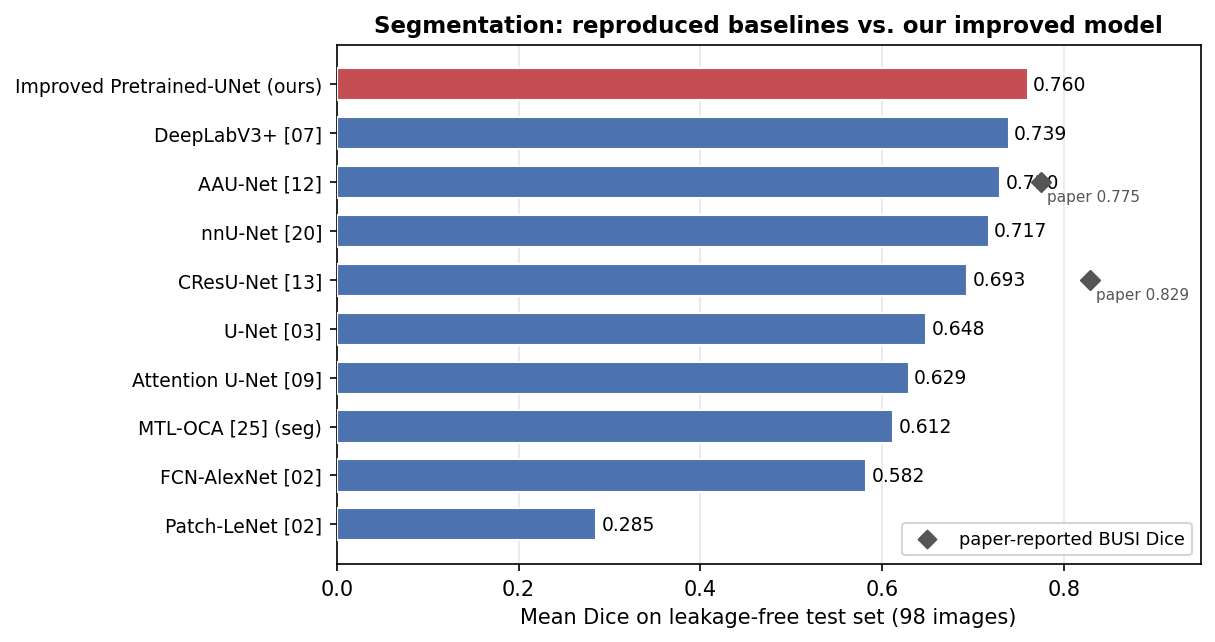
\includegraphics[width=0.88\linewidth]{fig_seg_dice_bar}
\caption{Segmentation Dice on the leakage-free test set. Our improved model (red)
leads; the two BUS-specific SOTA reproductions (AAU-Net, CResU-Net) fall below
their paper-reported Dice (diamonds) once near-duplicate leakage is removed.}
\label{fig:segbar}
\end{figure}

\paragraph{Ablation of the improved segmenter.}
Table~\ref{tab:abl} isolates the three ingredients. The result is unambiguous: the
ImageNet-pretrained encoder is responsible for essentially the \emph{entire} gain,
raising Dice from $0.648$ to $0.765$ ($+0.117$) and reducing the Dice standard
deviation from $0.362$ to $0.285$ -- i.e.\ far fewer completely-missed lesions.
Adding the Focal-Tversky loss does \emph{not} raise Dice (a marginal $-0.005$, from
$0.765$ to $0.760$); consistent with its design it raises pixel recall from
$0.763$ to $0.800$ at some cost to precision, shifting the operating point toward
not missing lesions rather than increasing overlap. TTA and post-processing give no
Dice gain on this data. We therefore explicitly \emph{do not} claim that
Focal-Tversky improves Dice; its measured effect is on recall.

\begin{table}[t]
\centering
\caption{Controlled ablation of the improved segmenter (test set, $98$ images).
Each row adds one component to the previous; everything else -- split,
pre-processing, augmentation, $60$ epochs, AdamW with cosine schedule -- is held
fixed. $\Delta$ is the change in Dice relative to the row above.}
\label{tab:abl}
\small
\begin{tabular}{@{}lccccccc@{}}
\toprule
Configuration & Dice & $\Delta$ & Dice $\sigma$ & IoU & Pix.\,P & Pix.\,R & FP/img \\
\midrule
From-scratch U-Net (Dice+BCE)               & 0.648 & --- & 0.362 & 0.570 & 0.775 & 0.637 & 0.296 \\
$+$ ImageNet-pretrained EffB4 encoder       & \best{0.765} & $+0.117$ & 0.285 & 0.685 & \best{0.799} & 0.763 & 0.214 \\
$+$ Focal-Tversky loss                       & 0.760 & $-0.005$ & \best{0.282} & 0.677 & 0.775 & \best{0.800} & 0.225 \\
$+$ TTA $+$ post-processing (full model)     & 0.760 & $\pm0.000$ & 0.307 & \best{0.688} & 0.765 & 0.790 & \best{0.163} \\
\bottomrule
\end{tabular}
\end{table}

Two details of Table~\ref{tab:abl} are worth reading carefully, because they are
easy to over-claim. First, the Focal-Tversky row is a genuine \emph{trade}, not a
wash: recall rises by $3.7$ points ($0.763\to0.800$) while precision falls by
$2.4$ ($0.799\to0.775$), and at the region level it recovers two further lesions
($86\to88$ true positives out of $98$). Dice, being symmetric in FP and FN, is
almost blind to this reallocation -- which is precisely why we report the
pixel-level breakdown rather than resting on the headline number. Second, the TTA
row leaves Dice unchanged but cuts false positives by a quarter ($0.225\to0.163$
per image) and lifts the detection F-measure from $0.846$ to $0.854$: the
largest-connected-component step deletes small spurious regions that contributed
too few pixels to register in Dice. Its Dice $\sigma$ nevertheless \emph{rises}
($0.282\to0.307$), because on images where the largest component is the wrong one,
discarding the rest converts a partial hit into a near-total miss. We therefore
keep TTA in the final model for its cleaner output while stating explicitly that
it does not improve overlap.

\paragraph{Qualitative and failure analysis.}
Figure~\ref{fig:segqual} shows representative predictions of the improved model:
compact, well-localised lesions are segmented accurately, but characteristic
failures remain -- small low-contrast lesions are partially missed (reducing
recall), fuzzy malignant boundaries are over- or under-segmented, and occasional
false-positive regions appear in shadowed tissue. The large Dice standard
deviation ($0.307$ for the full model; Table~\ref{tab:abl}) reflects a
sub-population of near-completely-missed lesions rather than a uniform small error,
which is why the pretrained encoder -- which most reduces that tail -- matters more
than boundary-level refinements.

\begin{figure}[t]
\centering
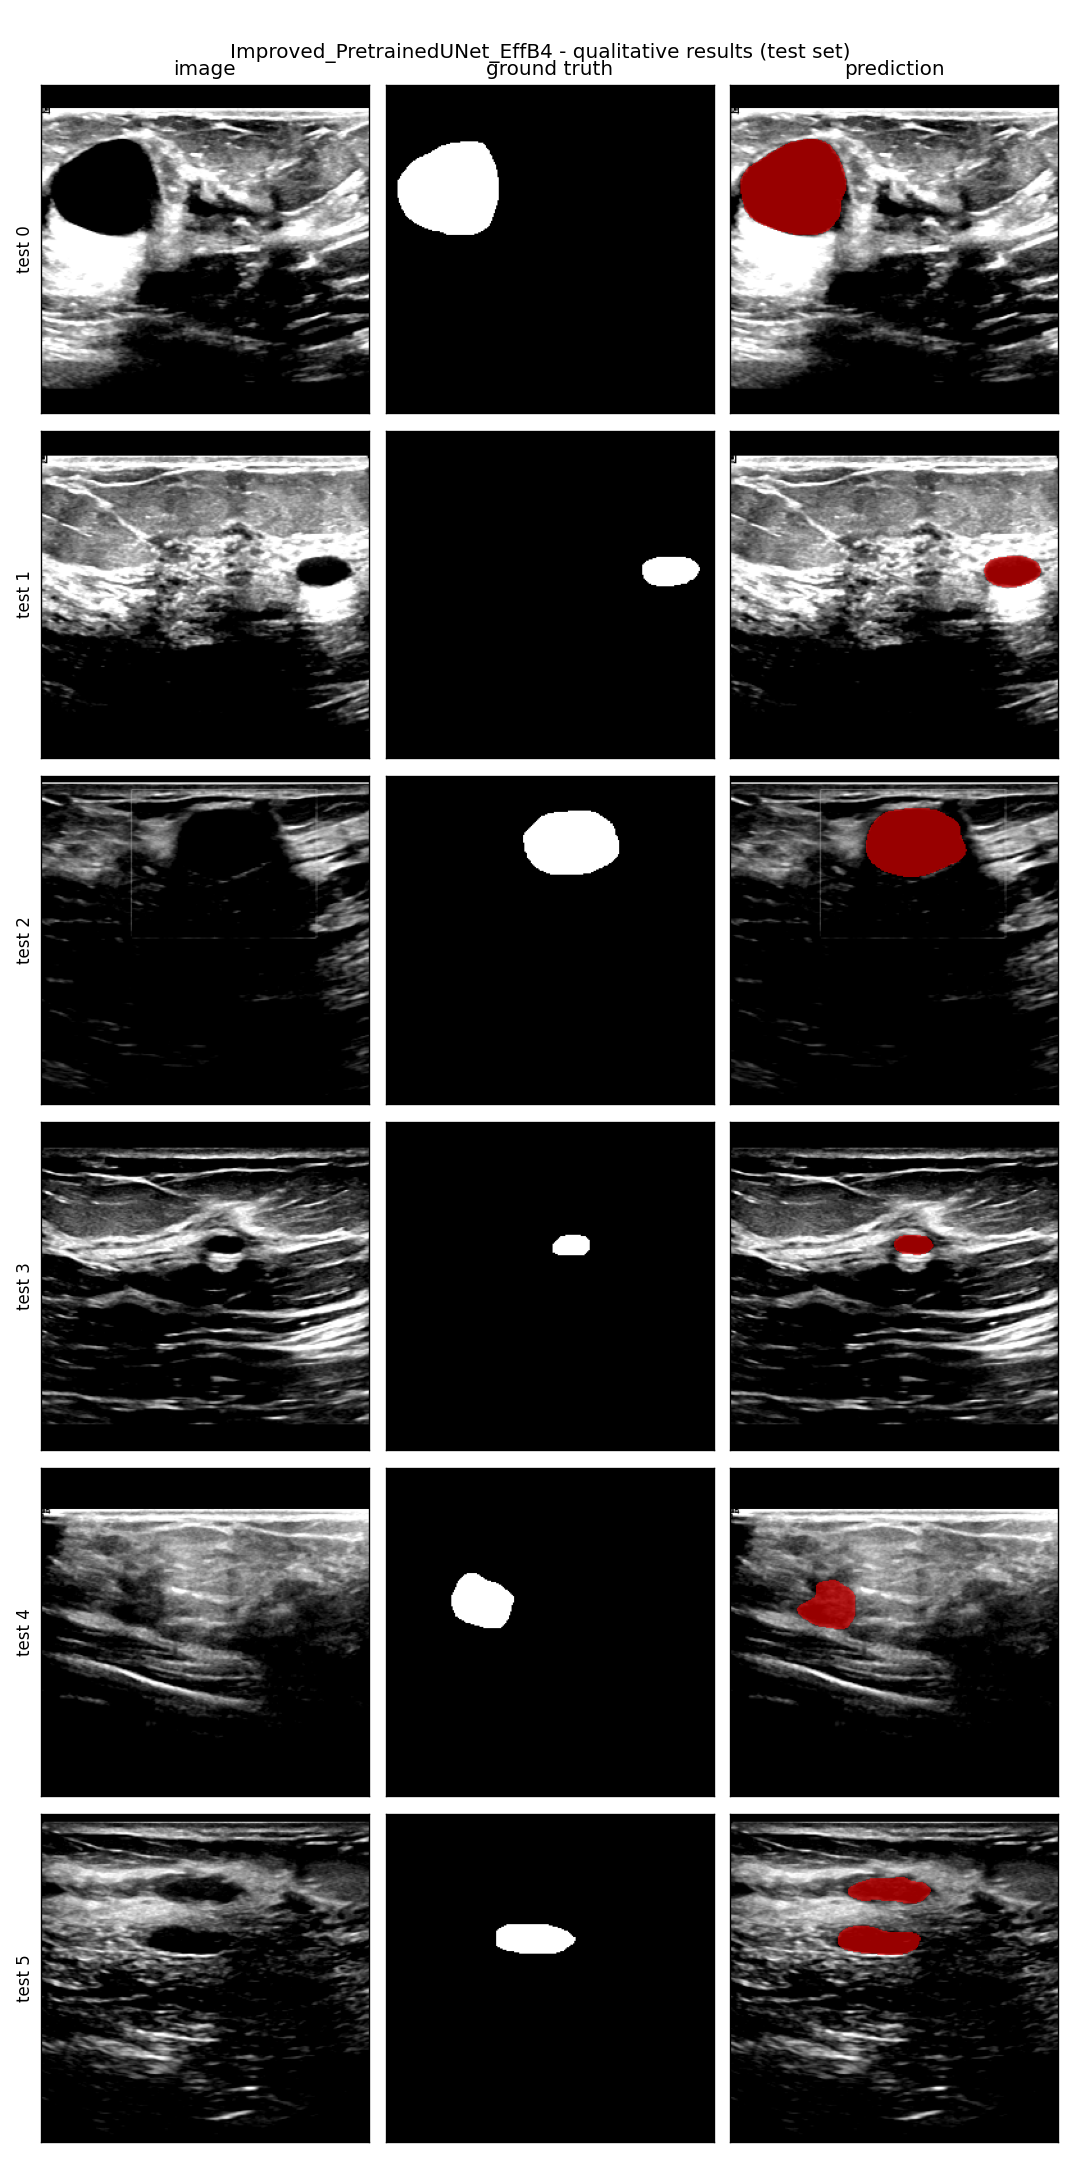
\includegraphics[width=0.8\linewidth,height=0.72\textheight, keepaspectratio]{Improved_PretrainedUNet_EffB4_examples}
\caption{Improved segmenter on test images (input, ground-truth mask, predicted
overlay). Compact lesions are captured well; small low-contrast lesions and fuzzy
malignant boundaries are the main failure modes.}
\label{fig:segqual}
\end{figure}

\subsection{Classification results}
\label{sec:results-cls}
Table~\ref{tab:cls} ranks the three-class classifiers by macro-F1. EfficientNet-B0
is best (macro-F1 $\best{0.828}$, AUC $0.969$), ahead of ResNet-18 ($0.810$) and
DenseNet-121 ($0.793$); all three pretrained backbones clearly beat the multi-task
MTL-OCA classifier ($0.720$). The confusion matrix of the best model
(Fig.~\ref{fig:cls}) shows the expected pattern: the minority \emph{malignant}
class is hardest and is the main source of error, and the residual confusion is
between benign and malignant (visually similar masses) and between normal and
benign. For EfficientNet-B0 the per-class F1 scores are normal $0.766$, benign
$0.884$ and malignant $0.833$, with malignant recall $0.807$; this per-class view,
not the overall accuracy ($0.848$), is the operative summary for an imbalanced
clinical task. MTL-OCA underperforms on \emph{both} tasks (segmentation $0.612$,
classification $0.720$), indicating that sharing one backbone across the two tasks
is, on this small dataset, worse than a specialised network per task.

\begin{table}[t]
\centering
\caption{Three-class classification on the leakage-free BUSI test set ($118$
images: $20$ normal, $67$ benign, $31$ malignant), ranked by macro-F1. Bal.\,acc.\
= balanced accuracy; AUC is macro one-vs-rest.}
\label{tab:cls}
\small
\begin{tabular}{@{}llccccc@{}}
\toprule
Model & Type & macro-F1 & Bal.\,acc. & Accuracy & AUC & min \\
\midrule
\best{EfficientNet-B0}~\cite{tan2019efficientnet} & transfer & \best{0.828} & \best{0.852} & \best{0.848} & \best{0.969} & \best{0.8} \\
ResNet-18~\cite{he2016resnet}      & transfer & 0.810 & 0.820 & 0.822 & 0.966 & 1.7 \\
DenseNet-121~\cite{huang2017densenet}& transfer & 0.793 & 0.804 & 0.805 & 0.947 & 1.4 \\
MTL-OCA~\cite{lu2025multitask} (cls)& joint    & 0.720 & 0.699 & 0.746 & 0.900 & 46.4 \\
\bottomrule
\end{tabular}
\end{table}

Table~\ref{tab:clsper} breaks the same runs down per class and shows that the
macro-F1 ranking hides genuinely different behaviour. \emph{Benign}, the majority
class, is easy for all three pretrained backbones (F1 $0.84$--$0.88$).
\emph{Malignant} is where they separate: EfficientNet-B0 is the most
\emph{precise} on malignant ($0.862$) but ResNet-18 is the most \emph{sensitive}
($R=0.839$ vs.\ $0.807$), catching one more of the $31$ malignant cases. Given
that a missed malignancy is the costliest error, ResNet-18 is arguably the better
operating point despite ranking second on macro-F1 -- a distinction that macro-F1
alone cannot express, and one that a deployment would resolve by tuning the
decision threshold rather than by swapping architectures.
\emph{Normal} is the noisiest class simply because it has $20$ test images, so each
one is worth $5$ percentage points of recall; EfficientNet-B0's high normal recall
($0.900$) comes with the lowest normal precision ($0.667$), i.e.\ it over-predicts
``normal'' and absorbs $9$ lesion images into it. MTL-OCA fails differently and
more seriously: its normal recall is only $0.600$, and $11$ of $67$ benign images
are called malignant, so sharing an encoder with the segmentation head costs it
most on exactly the distinction that matters clinically.

\begin{table}[t]
\centering
\caption{Per-class precision (P), recall (R) and F1 on the three-class test set.
Support: normal $20$, benign $67$, malignant $31$. Malignant recall, the
clinically critical quantity, is highlighted in the last column.}
\label{tab:clsper}
\small
\begin{tabular}{@{}l ccc ccc ccc c@{}}
\toprule
& \multicolumn{3}{c}{normal} & \multicolumn{3}{c}{benign} & \multicolumn{3}{c}{malignant} & \\
\cmidrule(lr){2-4}\cmidrule(lr){5-7}\cmidrule(lr){8-10}
Model & P & R & F1 & P & R & F1 & P & R & F1 & malig.\,R \\
\midrule
EfficientNet-B0 & 0.667 & \best{0.900} & 0.766 & \best{0.919} & \best{0.851} & \best{0.884} & \best{0.862} & 0.807 & \best{0.833} & 0.807 \\
ResNet-18       & 0.800 & 0.800 & 0.800 & 0.887 & 0.821 & 0.853 & 0.722 & \best{0.839} & 0.776 & \best{0.839} \\
DenseNet-121    & 0.773 & 0.850 & \best{0.810} & 0.859 & 0.821 & 0.840 & 0.719 & 0.742 & 0.730 & 0.742 \\
MTL-OCA (cls)   & \best{0.857} & 0.600 & 0.706 & 0.775 & 0.821 & 0.797 & 0.636 & 0.677 & 0.656 & 0.677 \\
\bottomrule
\end{tabular}
\end{table}

\begin{figure}[t]
\centering
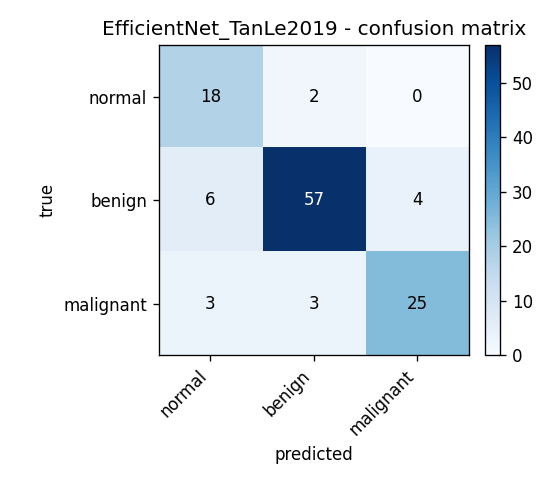
\includegraphics[width=0.44\linewidth]{EfficientNet_TanLe2019_confusion}
\caption{Confusion matrix of the best classifier (EfficientNet-B0, three-class
test set). Most error involves the minority malignant class and the
benign$\leftrightarrow$malignant boundary.}
\label{fig:cls}
\end{figure}

We did not generate Grad-CAM explanation maps for these classifiers in the current
result set, so we make no claim about where the classifier attends; producing and
auditing such maps is listed as future work (Section~\ref{sec:future}).

\subsection{Dual-stage results}
\label{sec:results-dual}
We separate exploratory single-run results (Table~\ref{tab:dual}a) from the
rigorous multi-seed results (Table~\ref{tab:dual}b, Fig.~\ref{fig:dualci}).

\emph{Controlled Stage-1 substitution.} Replacing Bruno's DeepLabV3+ Stage-1 with
our stronger segmenter raises Stage-1 Dice from $0.739$ to $0.760$ ($+0.021$) but
moves the single-run end-to-end macro-F1 only from $0.804$ to $0.807$ ($+0.003$).
Because the ROI coupling and the Stage-2 network, data and schedule are byte-for-byte
identical, this cleanly isolates the segmentation effect, and the transfer ratio is
about $0.14$ points of F1 per point of Dice -- an order of magnitude too small to
be worth optimising further.

The GT-ROI diagnostic explains why. Feeding the \emph{same} Stage-2 classifier
perfect ground-truth-mask crops lifts macro-F1 to $0.865$--$0.884$, so the
``Gap'' column of Table~\ref{tab:dual}a -- the score still recoverable by making
segmentation perfect -- is only $0.06$--$0.08$, and it does \emph{not} shrink when
Stage-1 improves (Bruno $0.061$, ours $0.077$). Even a hypothetical Dice-$1.0$
segmenter would leave the pipeline around $0.88$, which is within the confidence
interval of what we already achieve by ensembling alone (Table~\ref{tab:dual}b).
Put concretely, for the strengthened-Stage-2 row: the pipeline misclassifies $16$
of the $98$ test images and the GT-ROI oracle misclassifies $10$, so handing the
classifier perfect masks repairs six errors and leaves ten standing. The residual
error is therefore the classifier's own, on lesions that were
correctly localised -- the system is \emph{classifier-bound}, not
segmentation-bound (RQ3).

\emph{Rigorous evaluation.} The single-run ladder in Table~\ref{tab:dual}a looks
like a tidy climb ($0.804\to0.840$), but under out-of-fold training masks,
five-seed ensembling and bootstrap $95\%$ CIs (Table~\ref{tab:dual}b) the three
feature variants' intervals overlap almost entirely (Fig.~\ref{fig:dualci}).
Hand-crafted shape/texture features give \emph{no reliable} gain: the ensembles of
\emph{none} and \emph{shape} both reach $0.875$, and the per-seed means differ by
about one standard deviation. The only component that survives is
\emph{ensembling} (per-seed $0.847\to$ ensemble $0.875$). On a $98$-image test set,
single-run differences up to about $\pm0.05$ are not statistically resolved (RQ4).
Our best defensible dual-stage result is macro-F1 $\best{0.875}$ ($95\%$ CI
$[0.80,0.94]$).

\begin{table}[t]
\centering
\caption{Dual-stage pipelines on the two-class ($98$-image) test set
($67$ benign, $31$ malignant). (a)~single-run ladder (one seed each; indicative
only). (b)~rigorous evaluation with out-of-fold training masks, five-seed
ensembling and a bootstrap $95\%$ CI. (c)~the individual seeds behind~(b).
``GT-ROI'' is the perfect-segmentation upper bound (the same Stage-2 fed
ground-truth-mask crops); ``Gap'' is GT-ROI F1 minus pipeline F1, i.e.\ how much
score is still lost to imperfect segmentation. ``Malig.\,R'' is malignant recall.}
\label{tab:dual}
\smallskip
(a) single-run ladder --- differences are within test-set noise\\[2pt]
\scriptsize
\setlength{\tabcolsep}{4.4pt}
\begin{tabular}{@{}lccccccc@{}}
\toprule
Pipeline & Stage-1 Dice & Pipeline F1 & Accuracy & AUC & Malig.\,R & GT-ROI F1 & Gap \\
\midrule
Bruno (DeepLabV3+ $\to$ EffB0)~\cite{bruno2025dualstage} & 0.739 & 0.804 & 0.827 & 0.906 & 0.774 & 0.865 & $0.061$ \\
Ours: Improved-UNet Stage-1                              & 0.760 & 0.807 & 0.827 & 0.896 & 0.807 & 0.884 & $0.077$ \\
Ours: $+$ strengthened Stage-2                           & 0.760 & 0.817 & 0.837 & 0.905 & 0.807 & 0.882 & $0.065$ \\
Ours: $+$ shape features                                 & 0.761 & 0.840 & 0.857 & 0.936 & 0.839 & 0.850 & $0.010$ \\
\bottomrule
\end{tabular}
\smallskip

(b) rigorous: OOF cross-fitting $+$ 5-seed ensemble $+$ bootstrap $95\%$ CI ($B=2000$)\\[2pt]
\scriptsize
\setlength{\tabcolsep}{4.4pt}
\begin{tabular}{@{}lccccc@{}}
\toprule
Pipeline (rigorous) & Ensemble F1 & Per-seed mean$\pm$std & $95\%$ CI & Malig.\,R & GT-ROI F1 \\
\midrule
OOF $+$ no hand features (pure CNN) & \best{0.875} & $0.847\pm0.011$ & $[0.800,\,0.936]$ & \best{0.903} & 0.886 \\
OOF $+$ shape ($6$ feats)           & \best{0.875} & $0.861\pm0.016$ & $[0.800,\,0.936]$ & \best{0.903} & \best{0.906} \\
OOF $+$ radiomics ($14$ feats)      & 0.863 & $0.862\pm0.013$ & $[0.785,\,0.929]$ & 0.871 & 0.875 \\
\bottomrule
\end{tabular}
\smallskip

(c) individual seed scores behind panel (b) --- the spread that the single-run ladder hides\\[2pt]
\scriptsize
\begin{tabular}{@{}lccccc c@{}}
\toprule
Features & seed 0 & seed 1 & seed 2 & seed 3 & seed 4 & range \\
\midrule
none      & 0.857 & 0.830 & 0.838 & 0.855 & 0.855 & $0.027$ \\
shape     & 0.850 & 0.834 & 0.873 & 0.873 & 0.873 & $0.039$ \\
radiomics & 0.853 & 0.855 & 0.863 & 0.853 & 0.886 & $0.033$ \\
\bottomrule
\end{tabular}
\end{table}

Panel~(c) makes the argument concrete. Re-running the \emph{identical}
configuration with only the seed changed moves macro-F1 by up to $0.039$ --
comparable to the entire $0.036$ ``improvement'' of the single-run ladder in
panel~(a). The shape variant's own seeds span $0.834$ to $0.873$, so a study that
happened to report seed~2 and compare it against a no-feature seed~1 would
``show'' a $+0.043$ gain from shape features that is pure seed noise. This is the
mechanism by which single-run ablations on small medical datasets manufacture
findings, and it is why we treat panel~(a) as exploratory only. Ensembling behaves
as variance reduction should: for the two stronger configurations it lifts the
score \emph{above} the best individual seed (none: $0.857\to0.875$; shape:
$0.873\to0.875$), i.e.\ the ensemble is better than picking the luckiest run, not
merely better than the average one. For radiomics it lands at $0.863$, below that
configuration's best seed ($0.886$) but above its mean ($0.862$) -- the expected
behaviour when one seed is an outlier rather than genuinely better, and a further
reminder that a maximum over seeds is not a result.

\begin{figure}[t]
\centering
\begin{subfigure}{0.54\linewidth}
  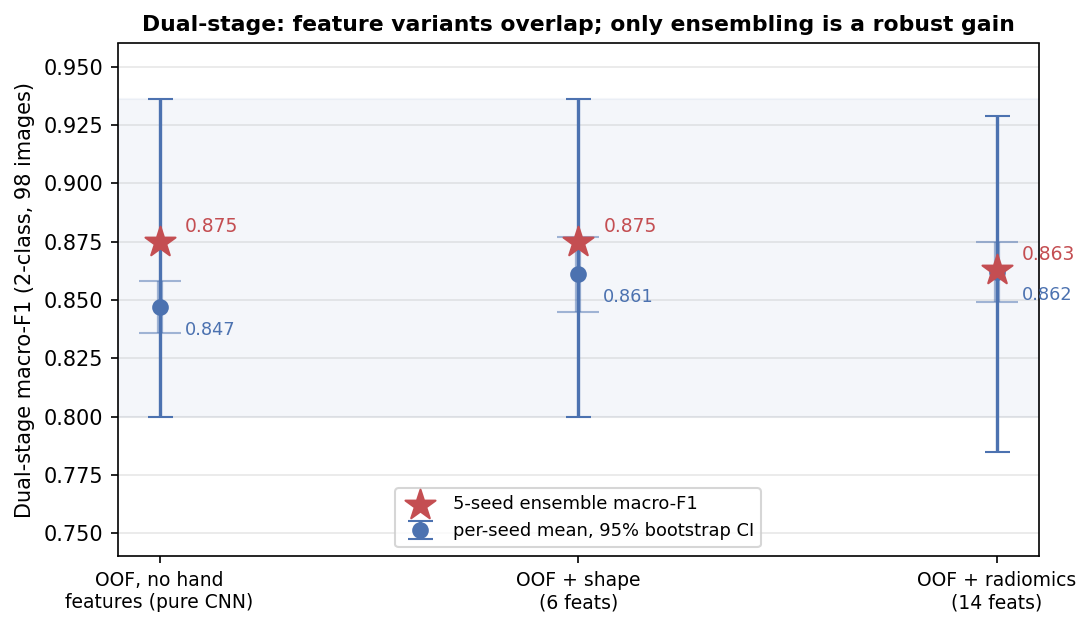
\includegraphics[width=\linewidth]{fig_dualstage_ci}
  \caption{Feature variants: per-seed CI vs.\ ensemble.}
  \label{fig:dualci}
\end{subfigure}\hfill
\begin{subfigure}{0.44\linewidth}
  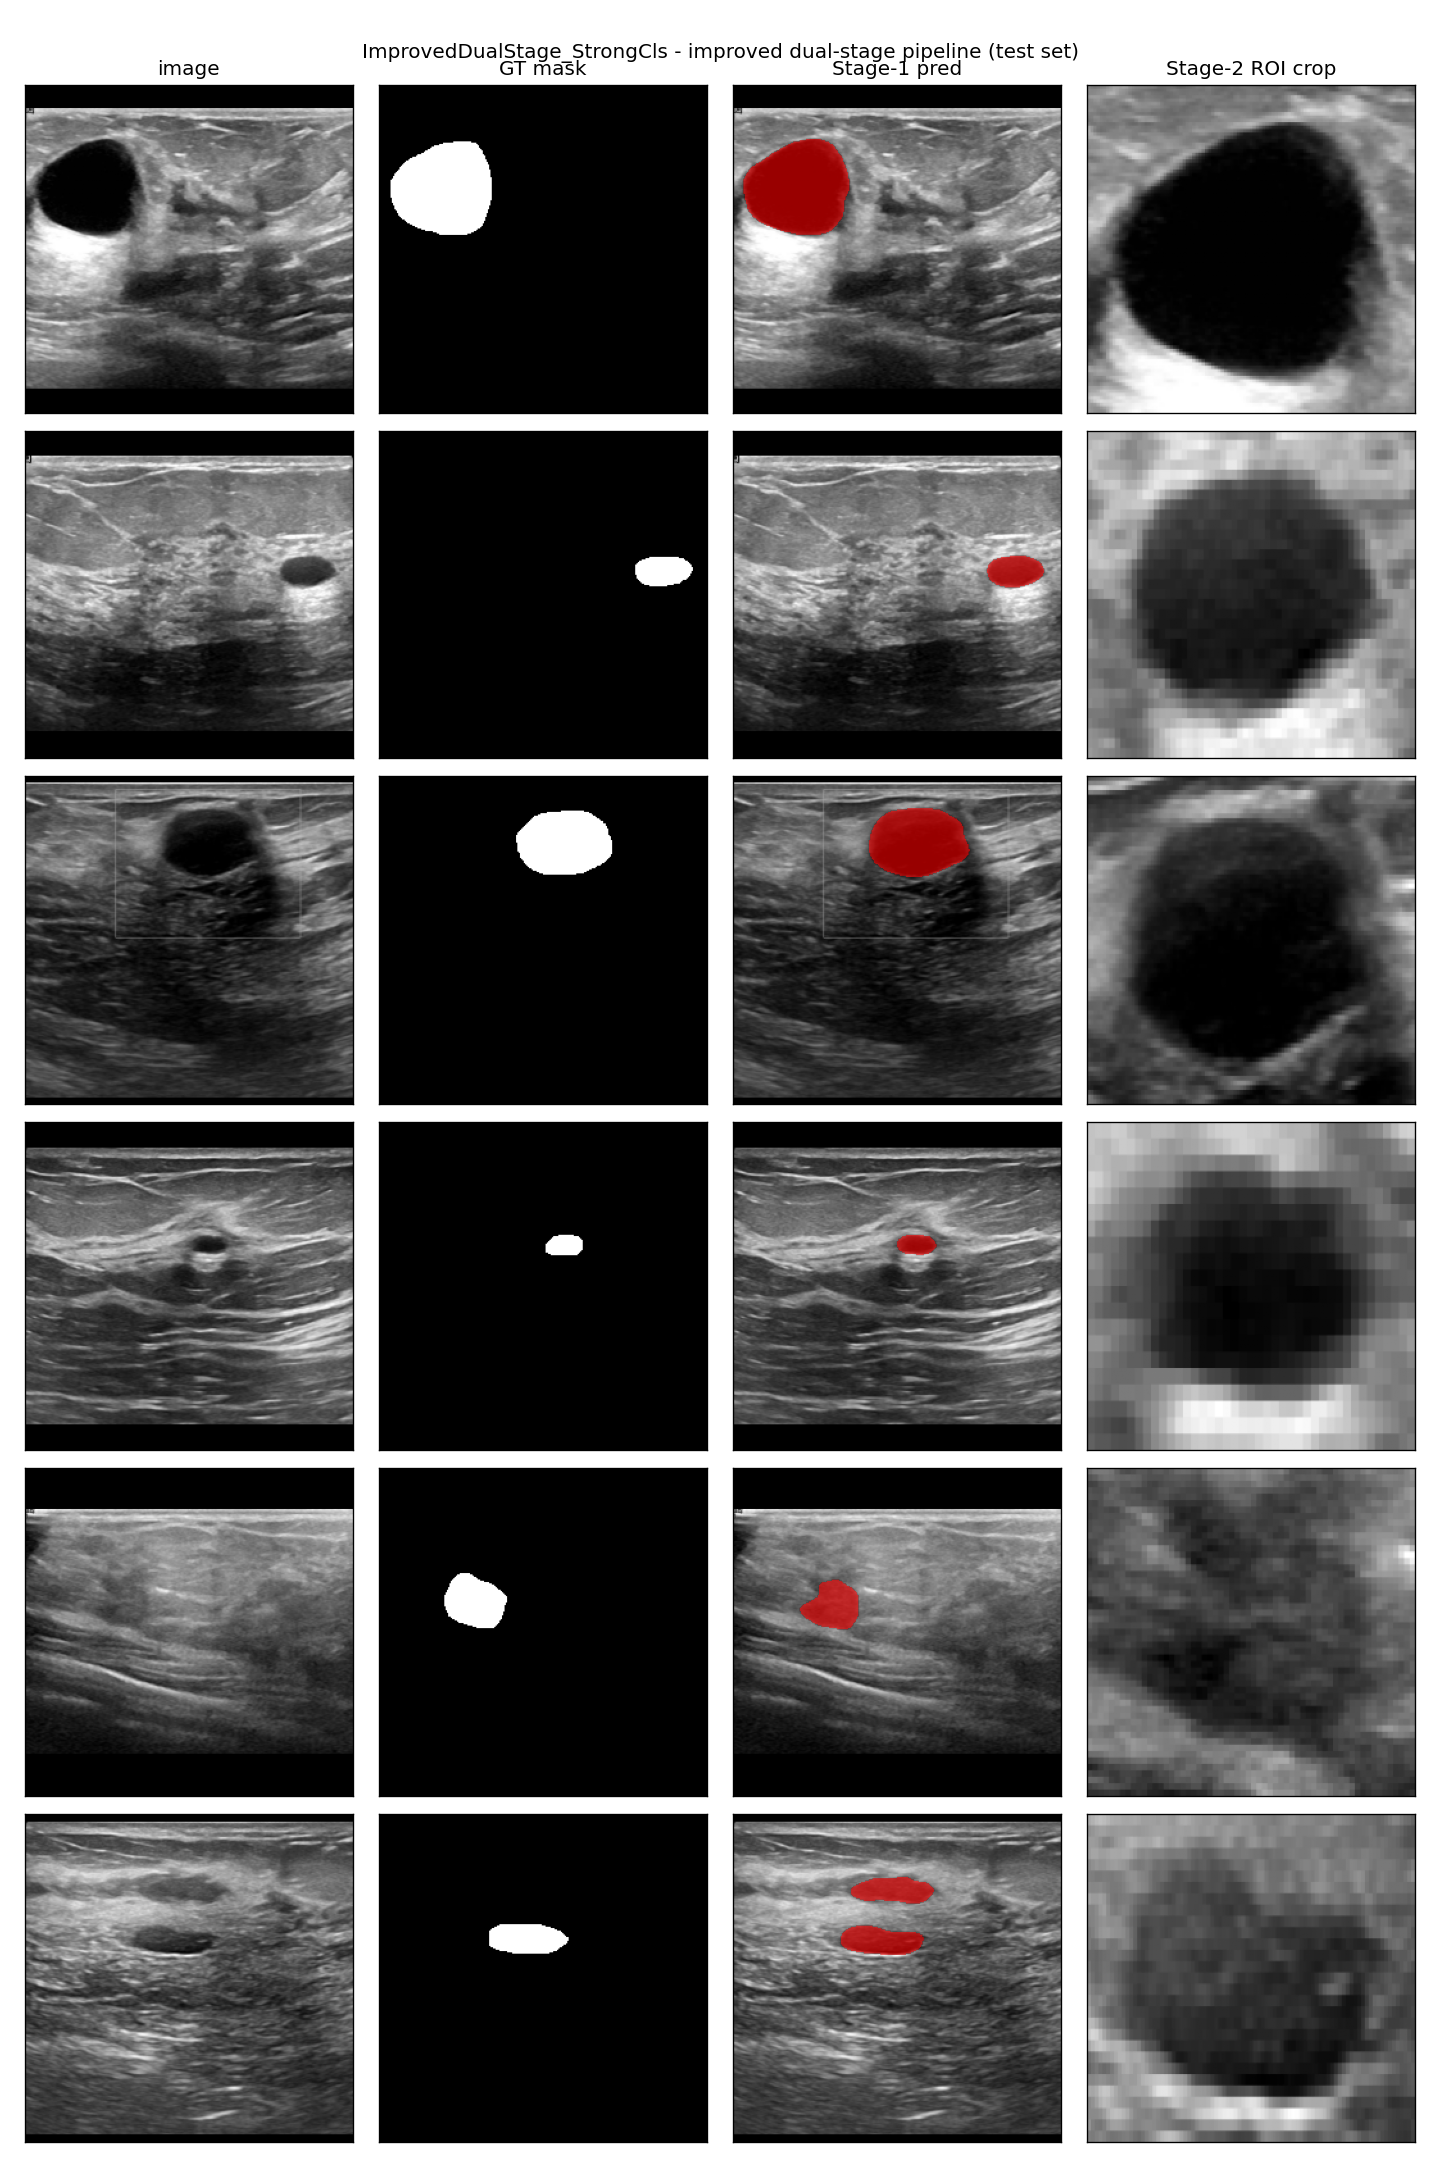
\includegraphics[width=\linewidth]{ImprovedDualStage_StrongCls_pipeline}
  \caption{Pipeline on test images.}
  \label{fig:dualpipe}
\end{subfigure}
\caption{Improved dual-stage pipeline. (a)~The three feature variants' $95\%$
confidence intervals overlap almost entirely; only ensembling (stars) reliably
lifts the per-seed mean (dots). (b)~Qualitative pipeline: input, ground-truth
mask, Stage-1 predicted mask, and the ROI crop passed to Stage-2.}
\label{fig:dual}
\end{figure}

\subsection{Error analysis}
\label{sec:results-error}
Across tasks the errors share a structure. In classification, the confusion is
concentrated on the malignant class and the benign$\leftrightarrow$malignant
boundary (Fig.~\ref{fig:cls}), which matches the EDA finding that benign and
malignant lesions overlap in intensity and can resemble one another
(Sections~\ref{sec:eda-img},~\ref{sec:eda-shape}); the small normal class is also
occasionally confused with benign. In segmentation, errors correlate with lesion
difficulty: small, low-contrast lesions and irregular malignant boundaries drive
the large Dice standard deviation, and the worst cases are near-complete misses
rather than uniform boundary error (Fig.~\ref{fig:segqual}). This is precisely the
sub-population the pretrained encoder most improves (Table~\ref{tab:abl}). In the
dual-stage pipeline, because the GT-ROI upper bound is close to the achieved score,
the remaining errors are classification errors on correctly localised lesions
rather than localisation failures. We report these patterns from the available
predictions and figures and do not select only favourable cases.

\subsection{Summary of research-question answers}
\label{sec:results-rq}
\textbf{RQ1:} under one leakage-free protocol, transfer-learned models lead each
task (segmentation: our improved U-Net $0.760$, DeepLabV3+ $0.739$;
classification: EfficientNet-B0 $0.828$); reproduced BUS-specific SOTA models score
below their reported numbers (AAU-Net $0.730$ vs.\ $0.775$; CResU-Net $0.693$ vs.\
$0.829$). \textbf{RQ2:} the pretrained encoder is decisive for segmentation
($+0.117$ Dice), while loss choice, attention gates, TTA and even nnU-Net add
little. \textbf{RQ3:} improving segmentation does \emph{not} reliably improve the
downstream pipeline; it is classifier-bound (GT-ROI upper bound sits far above the
achieved score). \textbf{RQ4:} apparent single-run gains are largely not stable --
only ensembling survives multi-seed and bootstrap evaluation (best macro-F1
$0.875$, $95\%$ CI $[0.80,0.94]$).

% =============================================================================
\section{Discussion}
\label{sec:discussion}
% =============================================================================
\subsection{Effect of evaluation hygiene}
The single most important factor shaping our numbers is evaluation hygiene. BUSI
contains roughly one third near-duplicate images and an exact cross-class
duplicate; a naive random split leaks visually identical frames across train and
test and inflates scores. Under our cluster-grouped, leakage-free split, reproduced
SOTA models fall well below their published values (CResU-Net $0.829\to0.693$ Dice;
AAU-Net $0.775\to0.730$). This does not mean our implementations are weak; it means
the published numbers were obtained without removing near-duplicates. Our results
are lower but trustworthy, and comparisons across papers that use different splits
and pre-processing should be treated cautiously. The practical implication is that
BUSI leaderboard numbers are not directly comparable unless the splitting and
de-duplication procedures match.

\subsection{Why transfer learning helped}
The controlled ablation (Table~\ref{tab:abl}) shows that an ImageNet-pretrained
encoder alone lifts Dice from $0.648$ to $0.765$ and sharply reduces
completely-missed lesions (std $0.362\to0.285$). The most plausible explanation is
that with only $445$ training images the network cannot learn robust low-level
visual features from scratch; a pretrained encoder supplies them and stabilises
optimisation, which also explains the much shorter training time
($58.5\to7.9$\,min). By contrast, a bespoke Focal-Tversky loss, test-time
augmentation, the attention gate of Attention U-Net and the self-configuring
nnU-Net add little \emph{overlap} here. We are careful not to over-generalise:
attention is not ineffective in general -- it simply did not improve performance
reliably in this project's small, noisy setting, where the dominant error is missed
lesions rather than imperfect boundaries. The Focal-Tversky loss is likewise not
useless -- it trades precision for higher lesion recall ($0.763\to0.800$), a
clinically sensible operating point -- but it does not raise Dice.

\subsection{Why the dual-stage pipeline was classifier-bound}
A much stronger Stage-1 barely moved the end-to-end score, and the
perfect-segmentation GT-ROI upper bound ($\approx 0.87$--$0.88$) sits far above the
achieved single-run score. Two things follow. First, a rough mask (Dice $0.76$) is
already good enough to crop a useful ROI, so segmentation is not the bottleneck.
Second, the residual error lives in Stage-2, so effort should go there. Our
strengthened Stage-2 -- trained on both ground-truth and predicted ROI crops to fix
the clean/imperfect distribution mismatch -- and, above all, ensembling are where
the gains came from. This is a transferable lesson about allocating
model-development effort: measure the bottleneck (here with a GT upper bound) before
investing in the more visible component.

\subsection{Statistical uncertainty}
The test set has only $98$ images, so single-seed rankings are unstable and small
differences are within noise. The bootstrap $95\%$ CIs are wide
($\approx[0.80,0.94]$) and overlap across the feature variants, which is exactly
why we decline to claim that shape or radiomics features help. Reporting per-seed
mean$\pm$std, an ensemble and a CI turns an over-confident single number into an
honest one, and it is the reason our headline dual-stage result is stated with its
interval. This is the project's central methodological contribution.

\subsection{Clinical and practical interpretation}
We interpret the system cautiously as \emph{decision support}, not autonomous
diagnosis. Because missing a malignancy is the costliest error, malignant recall
matters more than overall accuracy; the segmentation mask and ROI additionally
provide localisation and a degree of interpretability that a bare label lacks.
There is an inherent sensitivity/false-positive trade-off (the Focal-Tversky
operating point is one example), and the appropriate balance is a clinical, not
purely statistical, choice. None of the reported numbers, and none of the
wide-CI comparisons, would justify unsupervised clinical use.

\subsection{Limitations and threats to validity}
Several limitations qualify our conclusions. (i)~All results come from a single
small public dataset with one leakage-free split; even with OOF/multi-seed/CIs the
test set cannot resolve small differences. (ii)~There is no external, multi-centre
validation. (iii)~BUSI has near-duplicate and possible annotation issues (including
the cross-class conflict we removed). (iv)~We use static 2D frames, not full
ultrasound sequences, and the data carry acquisition/centre bias (lesion-centre
placement). (v)~Results are sensitive to pre-processing and thresholds, and our
hyper-parameter search was limited by compute. (vi)~Our reproductions may differ in
detail from the original implementations (for example loss or backbone
substitutions, noted per model), so the reproduced numbers characterise \emph{our}
faithful re-implementations under a common protocol rather than the original code.
(vii)~The dual-stage classification is two-class (benign/malignant) and is not
directly comparable to the three-class classifiers.

\subsection{Future work}
\label{sec:future}
The limitations point to concrete next steps: external and multi-centre validation;
full nested cross-validation under the same leakage-free protocol to remove any
remaining selection effect; uncertainty calibration and Grad-CAM auditing to check
that classifiers attend to the lesion rather than to artefacts; stronger or
ensembled ROI classifiers, since the pipeline is classifier-bound; ensemble or
self-supervised pretraining; adaptation of foundation-model segmenters such as
MedSAM under the same protocol; domain-generalisation across scanners; evaluation
on full ultrasound video rather than single frames; and a clinician-in-the-loop
assessment of the decision-support setting.

% =============================================================================
\section{Conclusion}
\label{sec:conclusion}
% =============================================================================
This project asked how established models perform on breast-ultrasound
classification and segmentation under a fair, leakage-free protocol; which design
choices matter; whether better segmentation improves downstream classification; and
whether apparent gains are statistically stable. To answer these, we detected
BUSI's near-duplicate images and built a cluster-grouped, leakage-free split, then
reproduced thirteen published models and added two of our own under this one
protocol. The evidence is consistent. Removing near-duplicate leakage lowers
published BUSI scores substantially (for example CResU-Net Dice $0.829\to0.693$),
so our numbers are lower but trustworthy (RQ1). For segmentation, transfer learning
is decisive: an ImageNet-pretrained encoder alone lifts Dice from $0.648$ to
$0.765$ and most reduces missed lesions, whereas a bespoke loss, attention gates,
test-time augmentation and nnU-Net add little; our improved pretrained U-Net is the
best segmenter overall (Dice $0.760$) (RQ2). For the combined task, a controlled
substitution and a ground-truth-ROI upper bound show the pipeline is bounded by its
classifier, not its segmenter (RQ3); and when candidate classifier improvements are
evaluated with out-of-fold training masks, five-seed ensembling and bootstrap
$95\%$ confidence intervals, the tidy single-run gains largely dissolve --
hand-crafted shape/texture features give no reliable improvement and only
ensembling survives, giving a best, defensible dual-stage macro-F1 of $0.875$
($95\%$ CI $[0.80,0.94]$) (RQ4). The central methodological contribution is thus a
discipline of honest evaluation on small medical datasets: remove leakage,
attribute gains with controlled ablations, and report multi-seed results with
confidence intervals. The principal limitation is that all findings rest on one
small dataset with a wide-interval test set, so external and multi-centre
validation is the essential next step. We present this as an experimental
decision-support study; it is not suitable for autonomous clinical diagnosis.

% =============================================================================
\begin{thebibliography}{99}
% =============================================================================
\bibitem{aldhabyani2020busi}
W.~Al-Dhabyani, M.~Gomaa, H.~Khaled, and A.~Fahmy,
``Dataset of breast ultrasound images,''
\emph{Data in Brief}, vol.~28, 104863, 2020.

\bibitem{yap2018cnn}
M.~H.~Yap et al.,
``Automated breast ultrasound lesions detection using convolutional neural networks,''
\emph{IEEE Journal of Biomedical and Health Informatics}, vol.~22, no.~4, pp.~1218--1226, 2018.

\bibitem{ronneberger2015unet}
O.~Ronneberger, P.~Fischer, and T.~Brox,
``U-Net: Convolutional networks for biomedical image segmentation,''
in \emph{MICCAI}, pp.~234--241, Springer, 2015.

\bibitem{he2016resnet}
K.~He, X.~Zhang, S.~Ren, and J.~Sun,
``Deep residual learning for image recognition,''
in \emph{CVPR}, pp.~770--778, 2016.

\bibitem{huang2017densenet}
G.~Huang, Z.~Liu, L.~van der Maaten, and K.~Q.~Weinberger,
``Densely connected convolutional networks,''
in \emph{CVPR}, pp.~4700--4708, 2017.

\bibitem{tan2019efficientnet}
M.~Tan and Q.~V.~Le,
``EfficientNet: Rethinking model scaling for convolutional neural networks,''
in \emph{ICML}, pp.~6105--6114, 2019.

\bibitem{chen2018deeplabv3plus}
L.-C.~Chen, Y.~Zhu, G.~Papandreou, F.~Schroff, and H.~Adam,
``Encoder-decoder with atrous separable convolution for semantic image segmentation,''
in \emph{ECCV}, pp.~801--818, 2018.

\bibitem{zhou2018unetpp}
Z.~Zhou, M.~M.~R.~Siddiquee, N.~Tajbakhsh, and J.~Liang,
``UNet++: A nested U-Net architecture for medical image segmentation,''
in \emph{DLMIA/ML-CDS Workshop, MICCAI}, pp.~3--11, Springer, 2018.

\bibitem{oktay2018attentionunet}
O.~Oktay et al.,
``Attention U-Net: Learning where to look for the pancreas,''
\emph{arXiv:1804.03999}, 2018.

\bibitem{huang2020unet3plus}
H.~Huang et al.,
``UNet~3+: A full-scale connected UNet for medical image segmentation,''
in \emph{ICASSP}, pp.~1055--1059, 2020.

\bibitem{chen2021transunet}
J.~Chen et al.,
``TransUNet: Transformers make strong encoders for medical image segmentation,''
\emph{arXiv:2102.04306}, 2021.

\bibitem{chen2023aaunet}
G.~Chen, L.~Li, Y.~Dai, J.~Zhang, and M.~H.~Yap,
``AAU-Net: An adaptive attention U-Net for breast lesions segmentation in ultrasound images,''
\emph{IEEE Transactions on Medical Imaging}, vol.~42, no.~5, pp.~1289--1300, 2023.

\bibitem{derakhshandeh2024cresunet}
M.~Derakhshandeh and A.~Mahloojifar,
``Modifying the U-Net's encoder-decoder architecture for segmentation of tumors in breast ultrasound images,''
\emph{Journal of Digital Imaging} (formerly arXiv:2409.00647), 2024.

\bibitem{latha2024effnetb7}
M.~Latha et al.,
``Revolutionizing breast ultrasound diagnostics with EfficientNet-B7 and Explainable AI,''
\emph{BMC Medical Imaging}, vol.~24, 230, 2024.

\bibitem{sulaiman2024attnbusi}
A.~Sulaiman et al.,
``Attention based UNet model for breast cancer segmentation using BUSI dataset,''
\emph{Scientific Reports}, vol.~14, 22422, 2024.

\bibitem{anari2025explainable}
S.~Anari et al.,
``Explainable attention based breast tumor segmentation using a combination of UNet, ResNet, DenseNet, and EfficientNet models,''
\emph{Scientific Reports}, vol.~15, 2025.

\bibitem{bruno2025dualstage}
A.~Bruno et al.,
``A dual-stage deep learning framework for breast ultrasound image segmentation and classification,''
\emph{Journal of Medical Systems}, 2025.

\bibitem{xian2018survey}
M.~Xian et al.,
``Automatic breast ultrasound image segmentation: A survey,''
\emph{Pattern Recognition}, vol.~79, pp.~340--355, 2018.

\bibitem{cheng2010survey}
H.~D.~Cheng et al.,
``Automated breast cancer detection and classification using ultrasound images: A survey,''
\emph{Pattern Recognition}, vol.~43, no.~1, pp.~299--317, 2010.

\bibitem{isensee2021nnunet}
F.~Isensee, P.~F.~Jaeger, S.~A.~A.~Kohl, J.~Petersen, and K.~H.~Maier-Hein,
``nnU-Net: A self-configuring method for deep learning-based biomedical image segmentation,''
\emph{Nature Methods}, vol.~18, pp.~203--211, 2021.

\bibitem{kirillov2023sam}
A.~Kirillov et al.,
``Segment Anything,''
in \emph{ICCV}, pp.~4015--4026, 2023.

\bibitem{ma2024medsam}
J.~Ma et al.,
``Segment Anything in medical images,''
\emph{Nature Communications}, vol.~15, 654, 2024.

\bibitem{selvaraju2017gradcam}
R.~R.~Selvaraju et al.,
``Grad-CAM: Visual explanations from deep networks via gradient-based localization,''
in \emph{ICCV}, pp.~618--626, 2017.

\bibitem{aldhabyani2019augmentation}
W.~Al-Dhabyani, M.~Gomaa, H.~Khaled, and A.~Fahmy,
``Deep learning approaches for data augmentation and classification of breast masses using ultrasound images,''
\emph{International Journal of Advanced Computer Science and Applications}, vol.~10, no.~5, 2019.

\bibitem{lu2025multitask}
Y.~Lu et al.,
``Automatic joint segmentation and classification of breast ultrasound images via multi-task learning with object contextual attention,''
\emph{Frontiers in Oncology}, vol.~15, 1567577, 2025.

\bibitem{salehi2017tversky}
S.~S.~M.~Salehi, D.~Erdogmus, and A.~Gholipour,
``Tversky loss function for image segmentation using 3D fully convolutional deep networks,''
in \emph{MICCAI MLMI Workshop}, pp.~379--387, 2017.

\bibitem{abraham2019focaltversky}
N.~Abraham and N.~M.~Khan,
``A novel focal Tversky loss function with improved attention U-Net for lesion segmentation,''
in \emph{IEEE ISBI}, pp.~683--687, 2019.

\bibitem{pawlowska2023}
A.~Paw{\l}owska, P.~Karwat, and N.~{\.Z}o{\l}ek,
``Letter to the Editor. Re: `Dataset of breast ultrasound images' by
W.~Al-Dhabyani, M.~Gomaa, H.~Khaled \& A.~Fahmy,
\emph{Data in Brief}, 2020, 28, 104863,''
\emph{Data in Brief}, vol.~48, 109247, 2023.
% NOTE: verify this entry against the publisher page before submission -- it is the
% only reference in this list not held as a PDF under papers/.

\end{thebibliography}

\end{document}
